\documentclass{beamer}
\usetheme{Copenhagen}
\usecolortheme{seahorse}
\usefonttheme[onlymath]{serif}

\usepackage{setspace}
\usepackage{xcolor}
\usepackage{graphicx}
\usepackage{multimedia}
\usepackage{fontawesome}
\usepackage{mathtools}
\usepackage{tikz}
\usetikzlibrary{positioning, calc, shapes.geometric, shapes.multipart, 
	shapes, arrows.meta, arrows, 
	decorations.markings, external, trees}
\tikzstyle{Arrow} = [
thick, 
decoration={
	markings,
	mark=at position 1 with {
		\arrow[thick]{latex}
	}
}, 
shorten >= 3pt, preaction = {decorate}
]

\newcommand{\blue}[1]{\textcolor{blue}{#1}}
\newcommand{\red}[1]{\textcolor{red}{#1}}
\newcommand{\violet}[1]{\textcolor{violet}{#1}}
\definecolor{ForestGreen}{RGB}{34,139,34}
\newcommand{\green}[1]{\textcolor{ForestGreen}{#1}}

\title[Data Fusion]{Fusion to address systematic errors across data sources}
\author[Paul Zivich]{Paul Zivich \\~\\ Department of Epidemiology \\ Causal Inference Research Laboratory \\ UNC Gillings School of Global Public Health}


\setbeamercovered{transparent}
\setbeamertemplate{navigation symbols}{}  % gets rid of the dumb navigation symbols
\setbeamertemplate{page number in head/foot}{\insertframenumber}  % adds slide #
\setbeamertemplate{headline}{}

\AtBeginSection[]{
	\begin{frame}
		\vfill
		\centering
		\begin{beamercolorbox}[sep=8pt,center,shadow=true,rounded=true]{title}
			\usebeamerfont{title}\insertsectionhead\par%
		\end{beamercolorbox}
		\vfill
	\end{frame}
}

\begin{document}

\begin{frame}[plain]
    \maketitle
\end{frame}

\begin{frame}{Acknowledgements}
	Supported by NIH T32-AI007001.\\~\\~\\
	
	Thanks to Stephen Cole, Jessie Edwards, Bonnie Shook-Sa, Alex Breskin, Michael Hudgens, and others at the UNC Causal Inference Research Lab (causal.unc.edu).\\~\\~\\
	
	Works in-progress, so errors are mine.\footnote[frame]{Footnotes are reserved for asides or references}\\~\\~\\
	
	\faEnvelope \quad pzivich@unc.edu \qquad \quad 
	\faGithub \quad pzivich \qquad \quad 
	\faTwitter \quad @PausalZ\\
\end{frame}

\section{Background}

\begin{frame}{Motivation}
	Recent developments in quantitative methods
	\begin{itemize}
		\item All promise to fundamentally improve how we learn
		\item Examples: causal inference, machine learning, big data
	\end{itemize}~\\
	However, study design remains the foundation
\end{frame}

\begin{frame}{Definitions of Fusion Study Designs}
	Combine heterogeneous data sources to answer a question that could not be answered (as well) by any subset\footnote[frame]{Cole et al. \textit{Am J Epi} (In-press)}~\\~\\
	\begin{itemize}
		\item Meta-analysis: combine 'similar' studies to reduce random error \\~\\
		\item Fusion: combine (possibly dissimilar) studies to reduce systematic and random error
	\end{itemize}
\end{frame}

\begin{frame}{A Visual Analogy}
	\centering		
	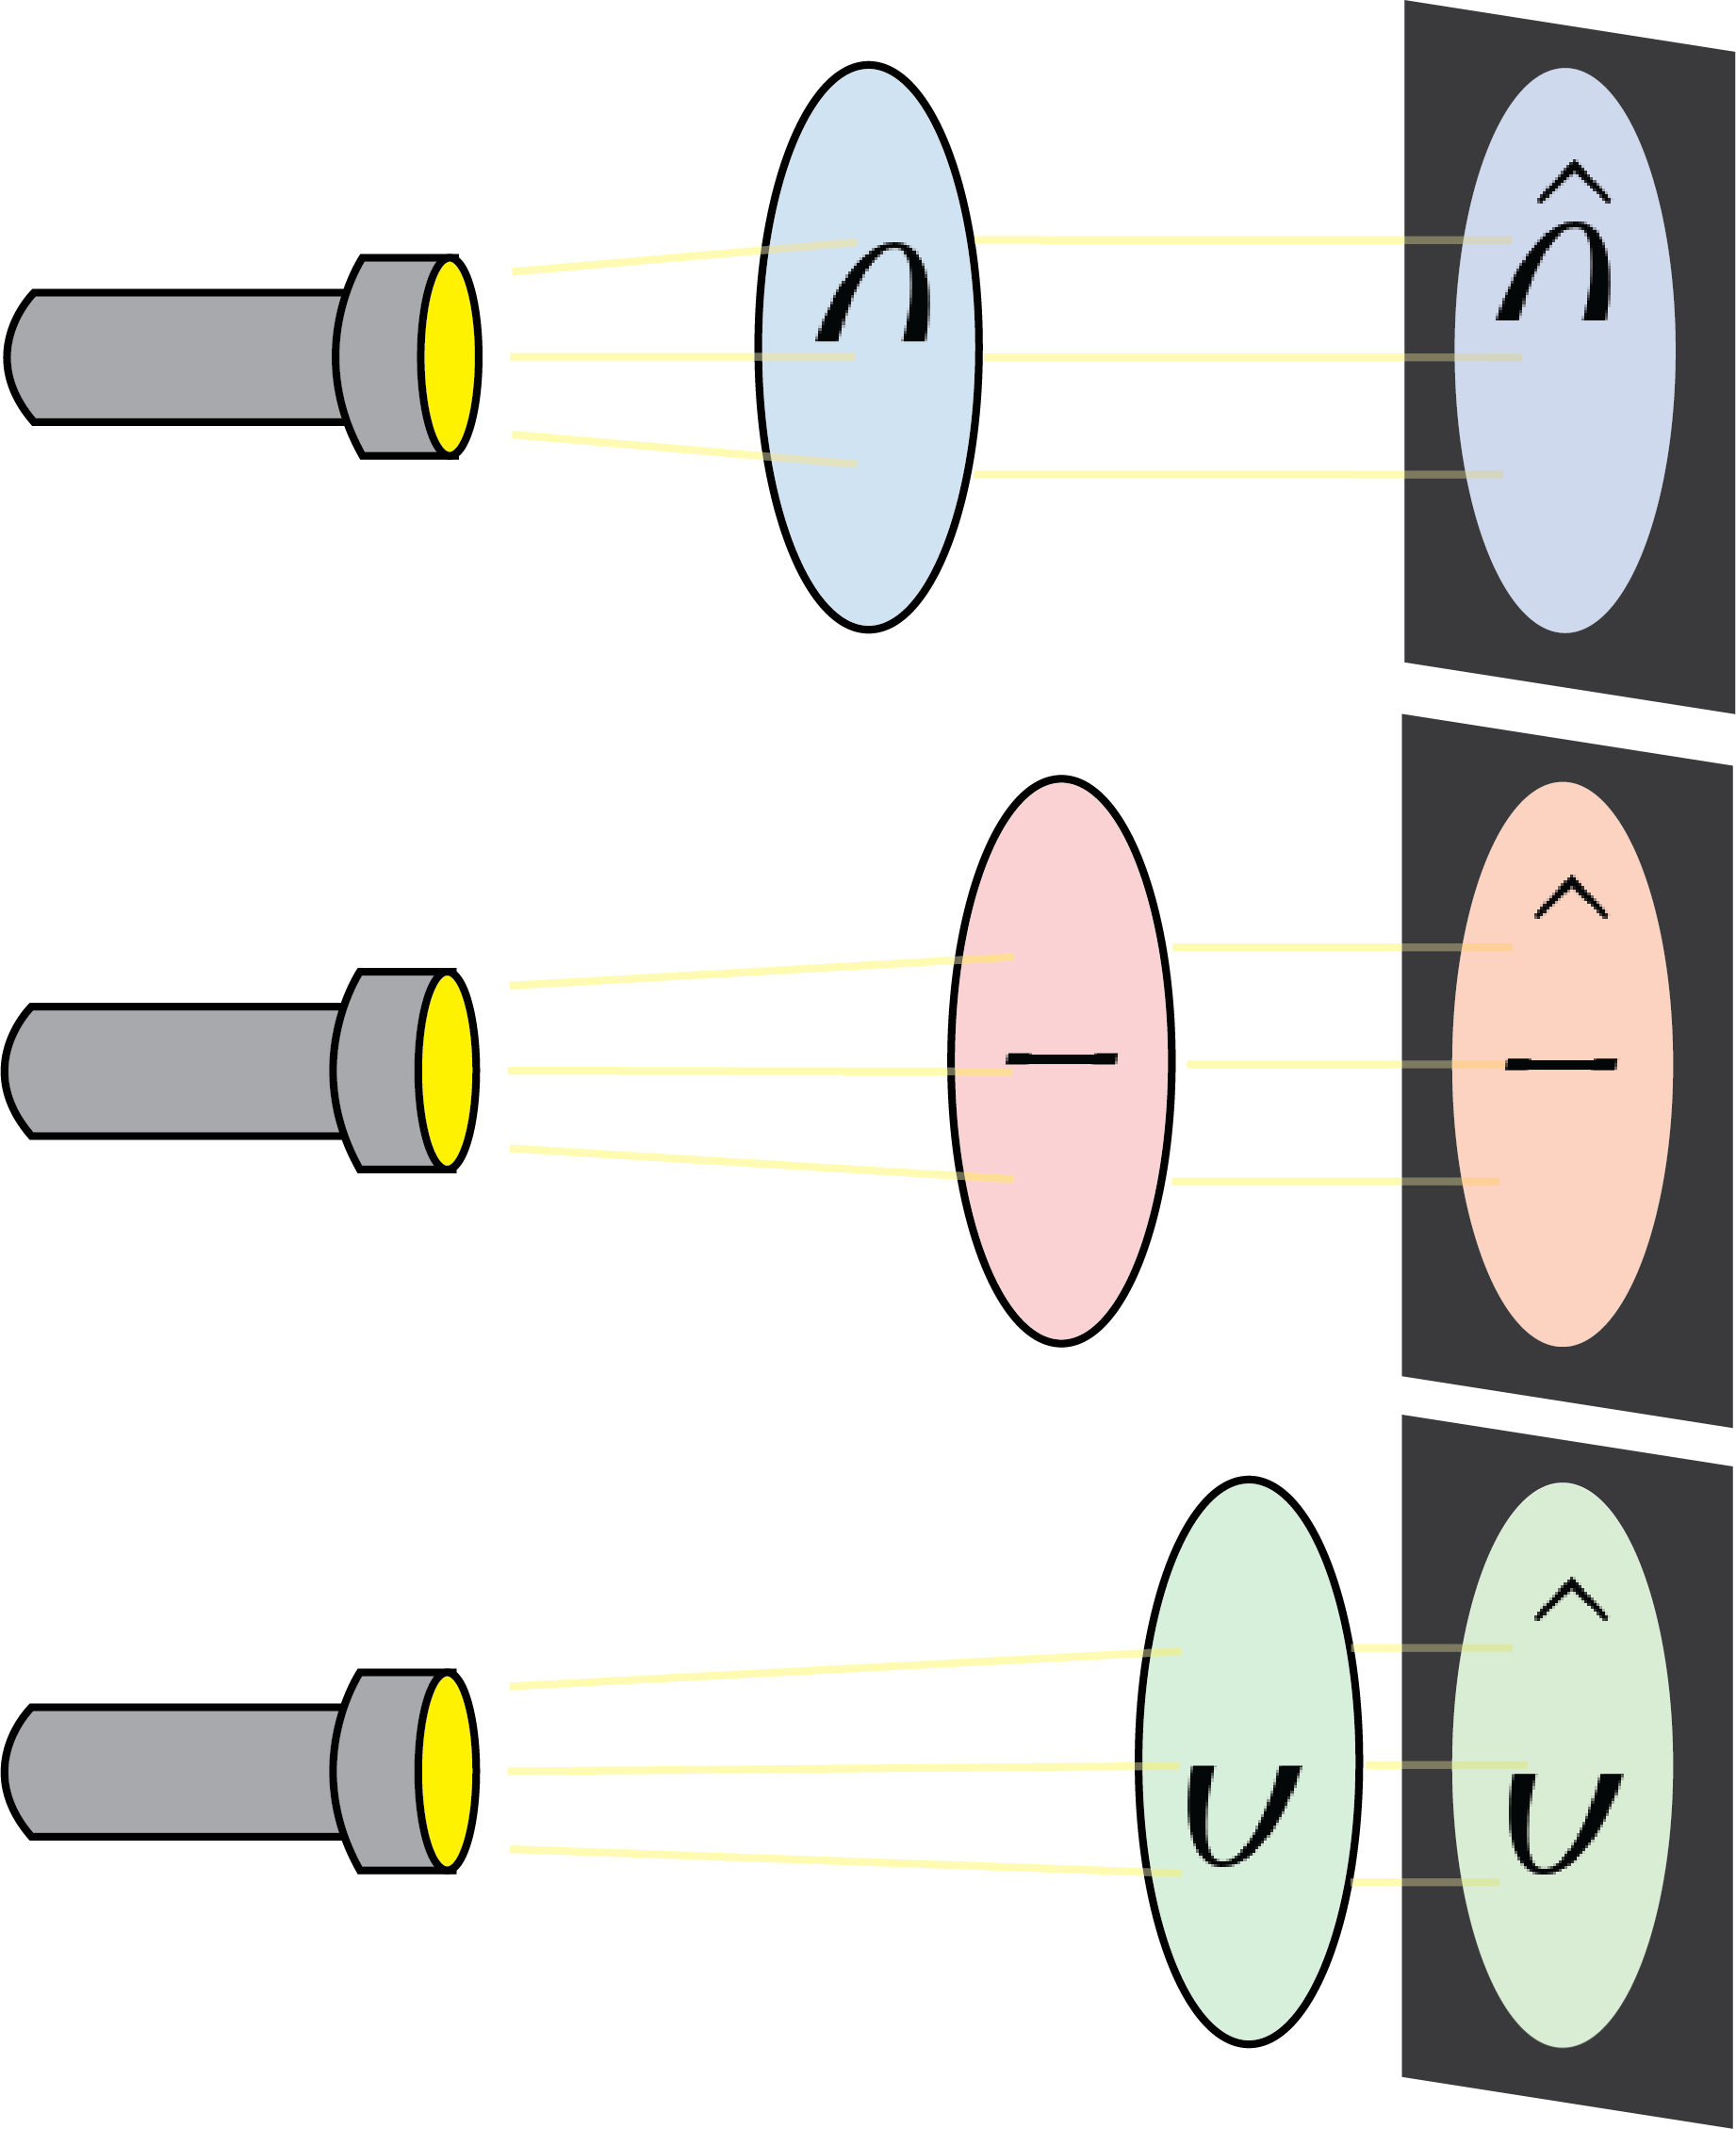
\includegraphics[scale=0.35]{images/fusion_piece_flashlight_analogy.png}	
\end{frame}

\begin{frame}{A Visual Analogy}
	\centering		
	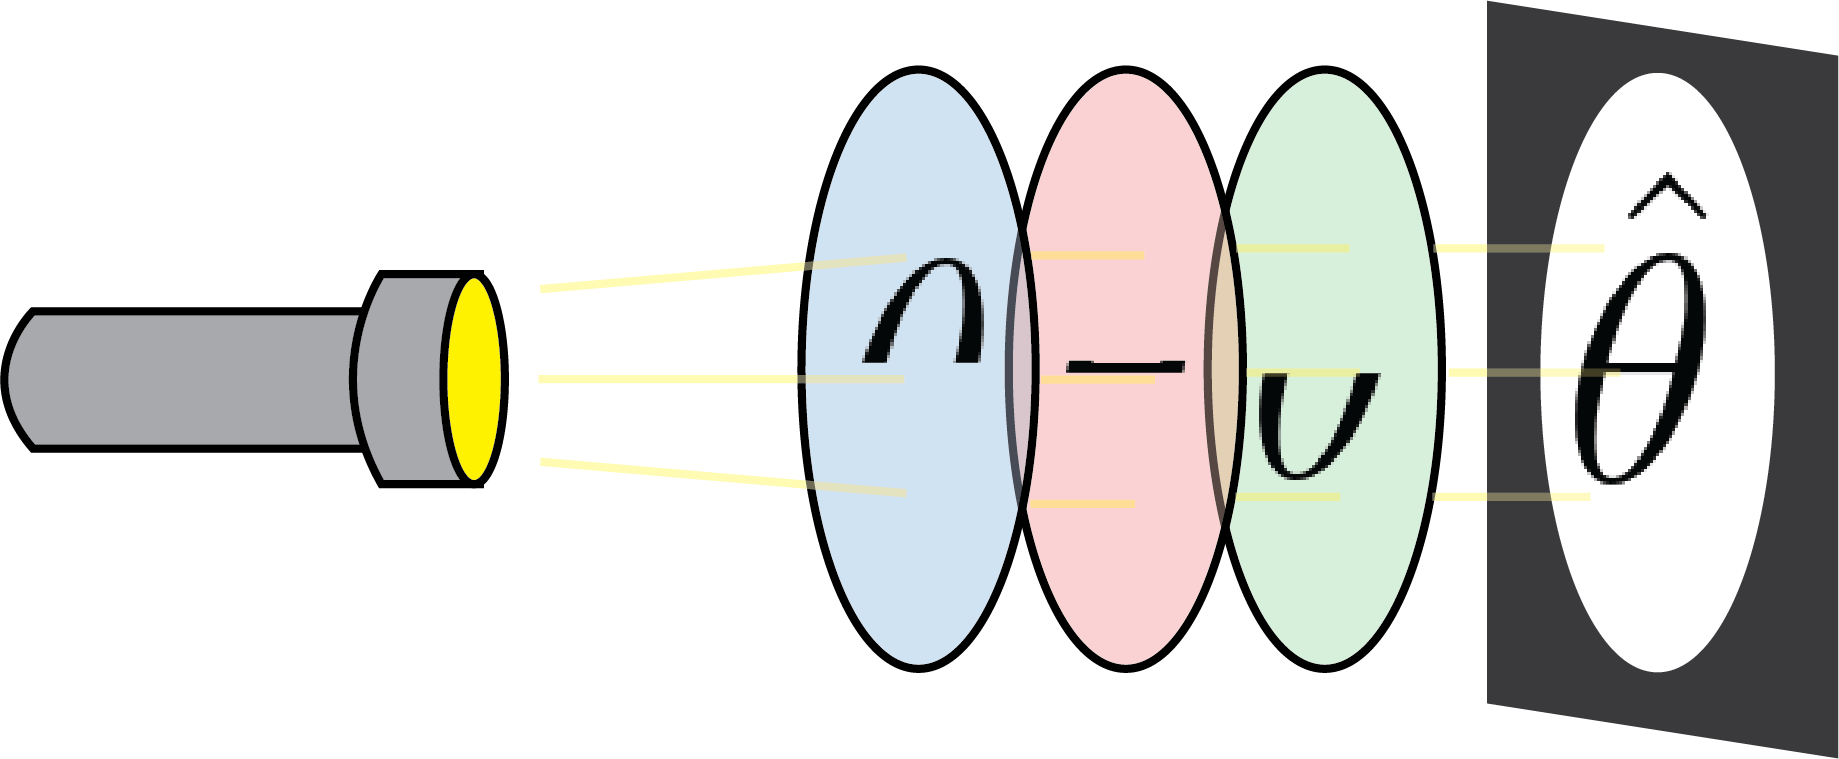
\includegraphics[scale=0.55]{images/fusion_analogy1.png}	
\end{frame}

\begin{frame}{A Visual Analogy}
	\centering
	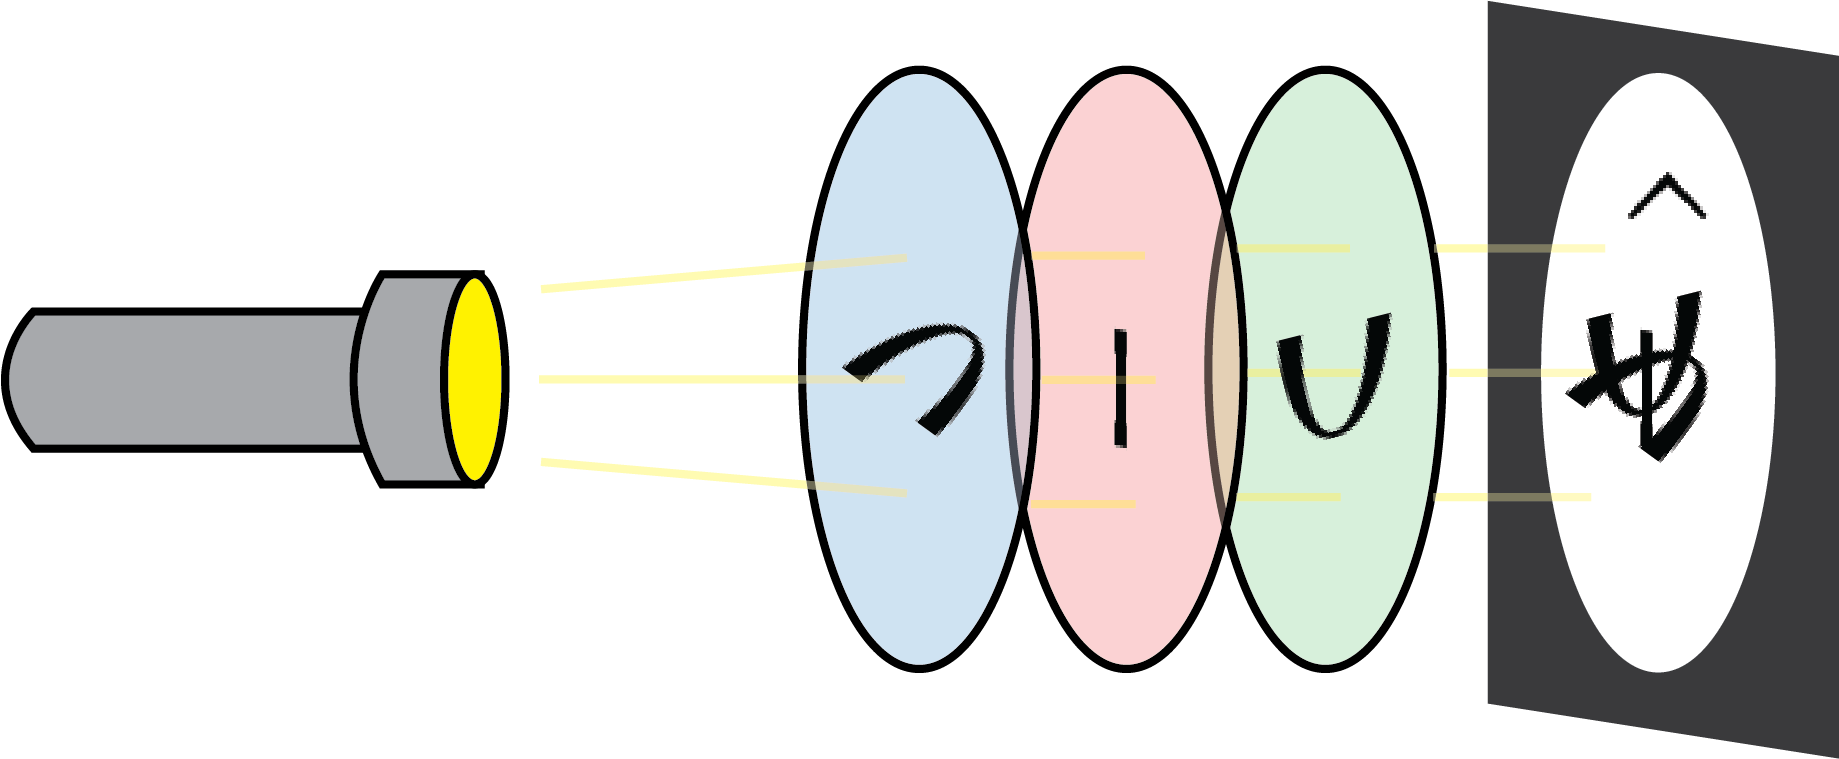
\includegraphics[scale=0.55]{images/fusion_analogy2.png}	
\end{frame}

\section{A Didactic Example}

\begin{frame}{Motivating Question}
	A collaborator asks us to help them estimate the mean of some variable ($Y$) for a defined population ($S=1$). However, $Y$ was not measured in the target population.\footnote[frame]{This problem is a simplified version of transportability}\\~\\~\\
	However, several sources of partially overlapping information are available\\~\\~\\
	So, under what assumptions could $\mu = E[Y|S=1]$ be estimated?\footnote[frame]{A variation of this is presented in Cole et al. (in-press) \textit{Am J Epidemiol}}
\end{frame}

\begin{frame}{Available Information}
	\begin{center}
		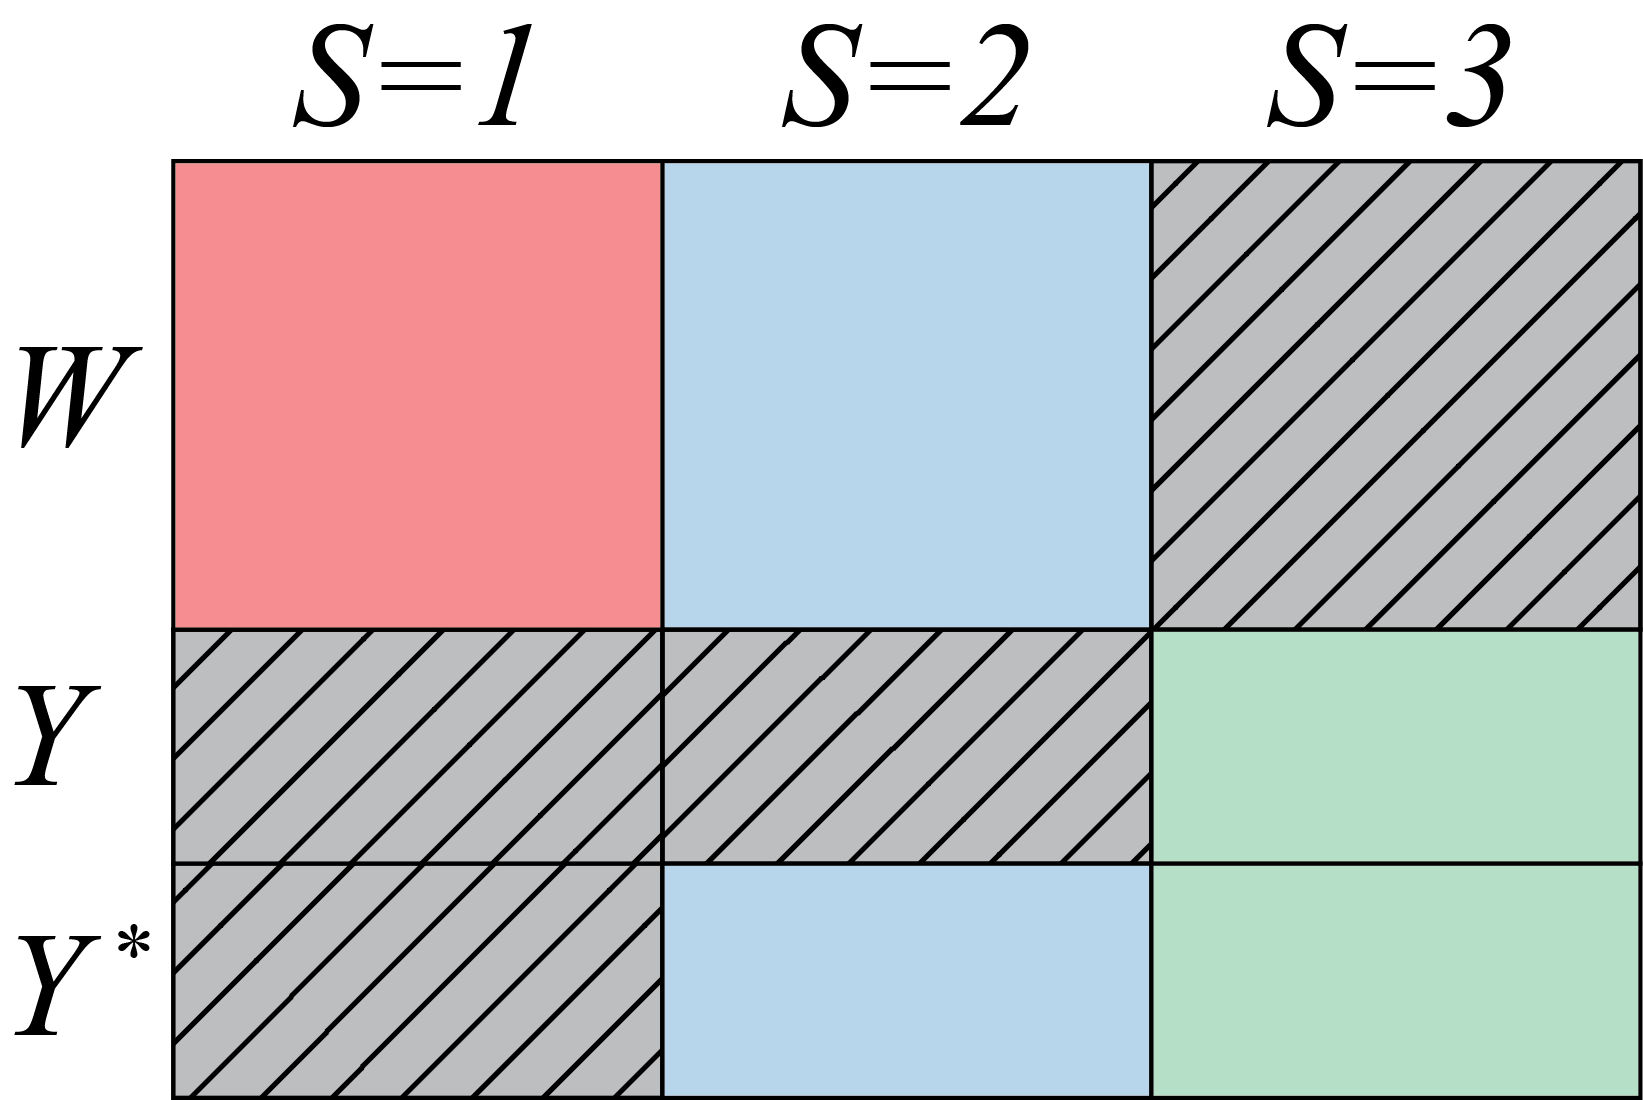
\includegraphics[scale=0.6]{code/data_sources.png}
	\end{center}
\end{frame}

\begin{frame}{Approach 1}
	\begin{minipage}[0.2\textheight]{\textwidth}
		\begin{columns}[T]
			\begin{column}{0.6\textwidth}
				Single data source: sample of $S=1$
				\begin{itemize}
					\item $Y$ not measured
					\item So can make no further progress
				\end{itemize}~\\
				\[\hat{\mu}_1 = \varnothing\]
			\end{column}
			\begin{column}{0.35\textwidth}
				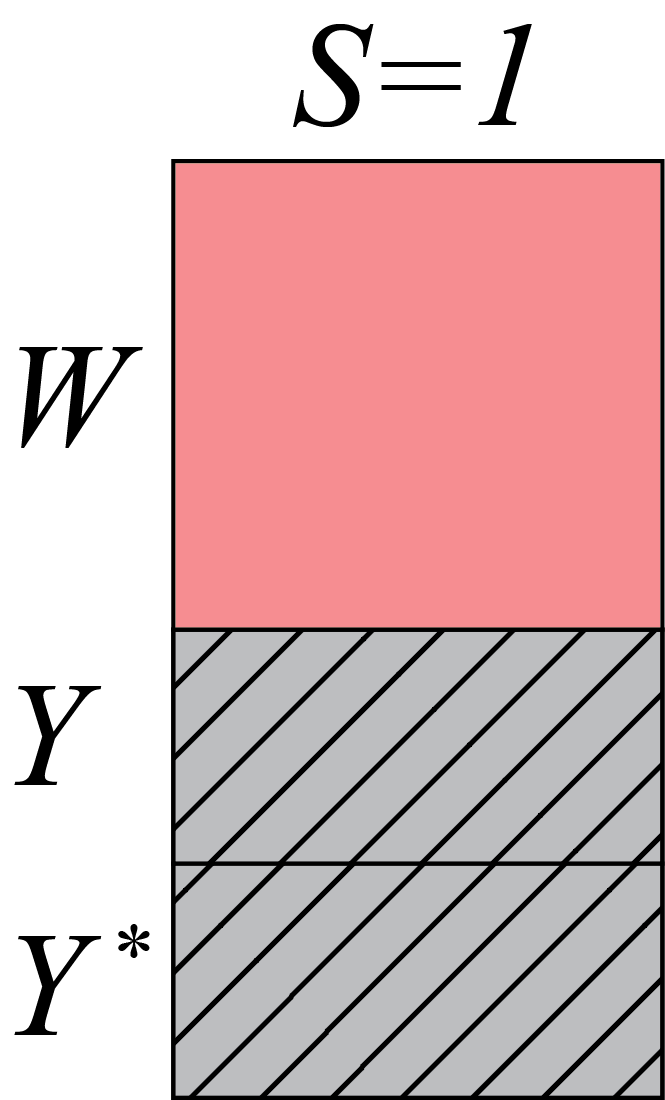
\includegraphics[width=3.5cm]{images/data_sources1.png}
			\end{column}
		\end{columns}
	\end{minipage}	
\end{frame}

\begin{frame}{Approach 2}
	\begin{minipage}[0.2\textheight]{\textwidth}
		\begin{columns}[T]
			\begin{column}{0.6\textwidth}
				Single data source: sample of $S=2$
				\begin{itemize}
					\item $Y$ not measured
					\item Mismeasured $Y$, $Y^*$, is available
				\end{itemize}~\\
				Assumptions\footnote[frame]{Webster-Clark \& Breskin (2021) \textit{Am J Epidemiol}}
				\begin{itemize}
					\item $Y = Y^*$
					\item $E[Y | S=1] = E[Y | S=2]$
				\end{itemize}~\\
				\[\hat{\mu}_2 = n_2^{-1} \sum_i I(S_i = 2) Y_i^*\]
			\end{column}
			\begin{column}{0.35\textwidth}
				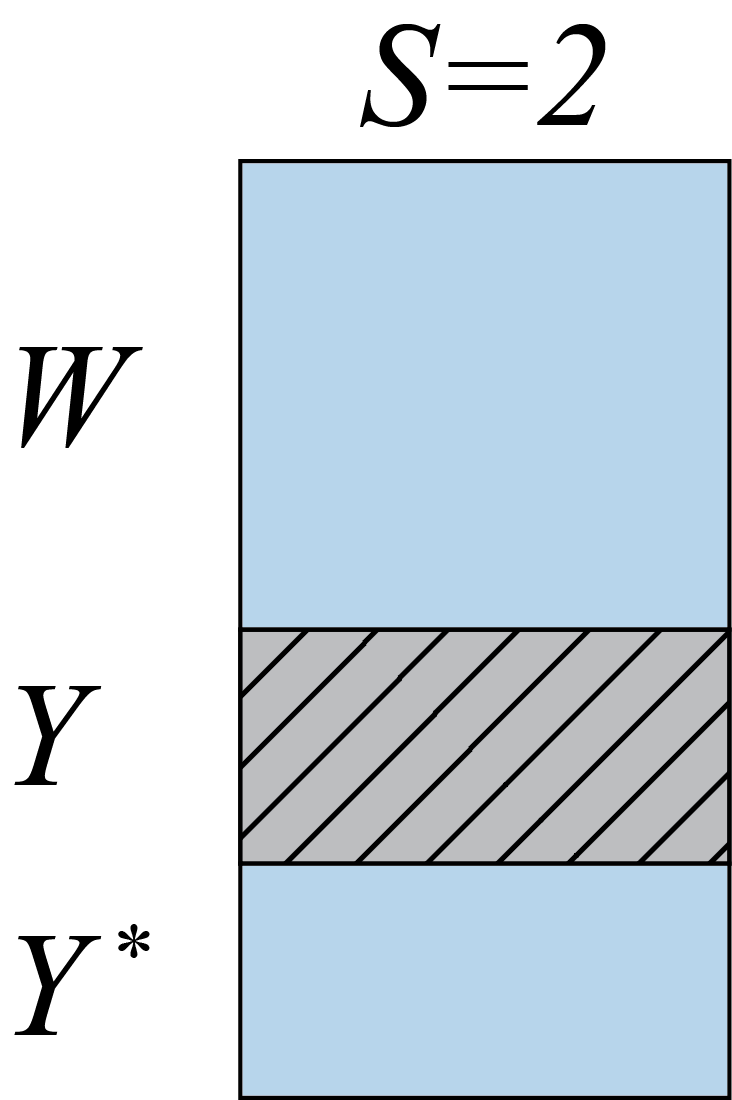
\includegraphics[width=3.5cm]{images/data_sources2.png}
			\end{column}
		\end{columns}
	\end{minipage}	
\end{frame}

\begin{frame}{Approach 3}
	\begin{minipage}[0.2\textheight]{\textwidth}
		\begin{columns}[T]
			\begin{column}{0.6\textwidth}
				Single data source: sample of $S=3$
				\begin{itemize}
					\item $Y$ and $Y^*$ were measured
				\end{itemize}~\\
				Assumptions
				\begin{itemize}
					\item $E[Y | S=1] = E[Y | S=3]$
				\end{itemize}~\\
				\[\hat{\mu}_3 = n_3^{-1} \sum_i I(S_i = 3) Y_i\]
			\end{column}
			\begin{column}{0.35\textwidth}
				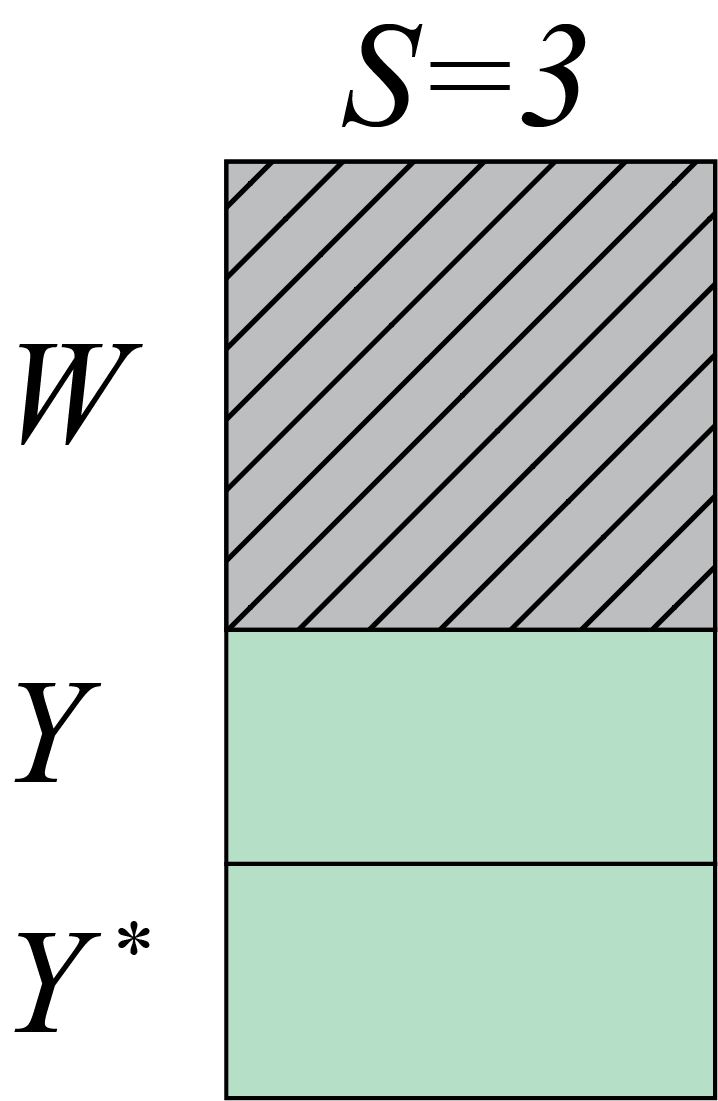
\includegraphics[width=3.5cm]{images/data_sources3.png}
			\end{column}
		\end{columns}
	\end{minipage}	
\end{frame}

\begin{frame}{Fusion (Approach 4)}
	\begin{minipage}[0.2\textheight]{\textwidth}
		\begin{columns}[T]
			\begin{column}{0.6\textwidth}
				All data sources
				\begin{itemize}
					\item Sample of $S=1$
					\begin{itemize}
						\item Contribute $W$
					\end{itemize}
					\item Sample of $S=2$
					\begin{itemize}
						\item Contribute $W,Y^*$
						\item Measure of $Y$ conditional on $W$
					\end{itemize}
					\item Sample of $S=3$
					\begin{itemize}
						\item Contribute $Y,Y^*$
						\item Account for measurement error
					\end{itemize}
				\end{itemize}~\\
				Not enough
				\begin{itemize}
					\item Need to combine data sources correctly
				\end{itemize}	
			\end{column}
			\begin{column}{0.35\textwidth}
				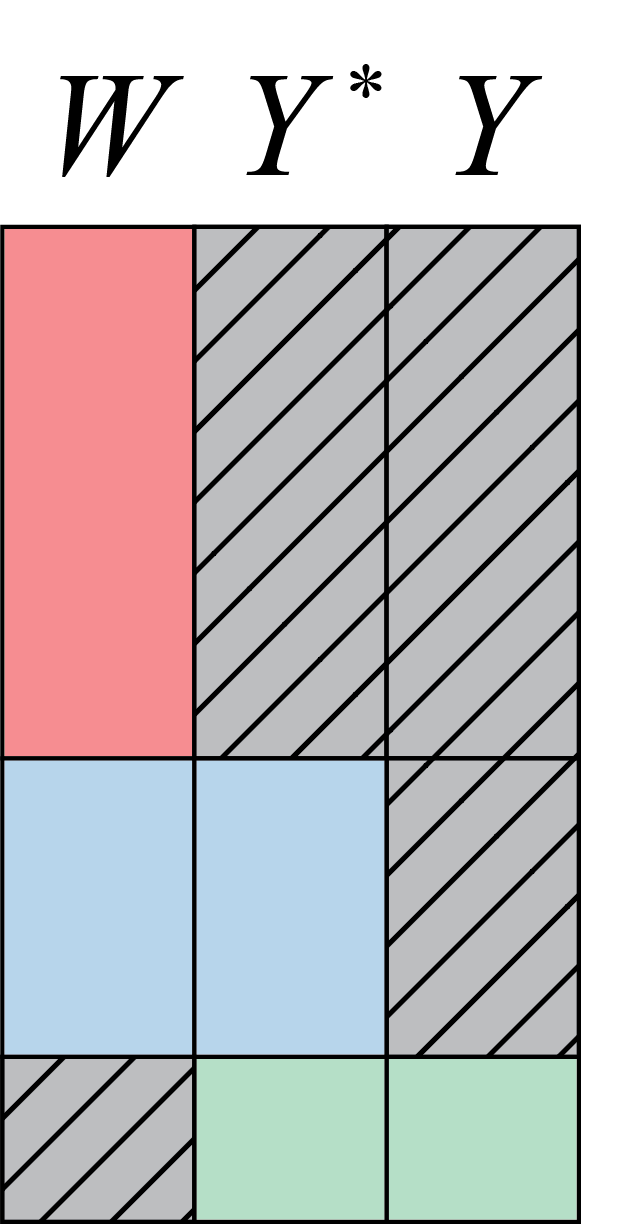
\includegraphics[width=3.5cm]{images/data_sources4.png}
			\end{column}
		\end{columns}
	\end{minipage}	
\end{frame}

\begin{frame}{Fusion: Identification}
	Link $S=1$ and $S=2$:
	\begin{itemize}
		\item Conditional transportability assumptions\footnote[frame]{Westreich et al. (2017) \textit{Am J Epidemiol}}
	\end{itemize}
	$$E[Y | W, S=1] = E[Y | W, S=2]$$
	$$\Pr(S=2 | W=w) > 0 \text{ where } \Pr(S=1 | W=w) > 0$$
	~\\~\\
	Link $S=2$ and $S=3$:
	\begin{itemize}
		\item Non-differential measurement error
	\end{itemize}
	$$\Pr(Y^*=y|Y=y) = \Pr(Y^*=y|Y=y,W=w)$$
\end{frame}

\begin{frame}{Fusion: Estimation}
	M-estimator:\footnote[frame]{See Stefanski \& Boos (2002) \textit{Am Stat} for an introduction}~\\
	\[\sum_{i=1}^{n} \psi(O_i; \hat{\theta}) = 0\]~\\~\\
	where $O_i = \{S_i, W_i, Y_i, Y_i^*\}$ and $\theta = (\mu, \eta)$
	% Like our 'stacked' data sets, we can 'stack' our estimating equations
\end{frame}

\begin{frame}{Fusion: Estimation}
	Stacked estimating equation\footnote[frame]{Measurement correction from Rogan \& Gladen (1978) \textit{Am J Epidemiol}}
	$$ \psi(O_i; \theta) =
	\left[
	\begin{matrix}
		\green{I(S_i=3) \; Y_i \; (Y_i^* - \eta_1)} \\		
		\green{I(S_i=3) (1 - Y_i) \left((1-Y_i^*) - \eta_2\right)}\\
		\violet{I(S_i \ne 3) \left(I(S_i=1) - \text{expit}(W_i \beta)\right)W_i}\\
		\blue{I(S_i = 2) (Y_i^* - \eta_3) \frac{1 - \text{expit}(W_i \beta)}{\text{expit}(W_i \beta)}}\\
		\mu (\eta_1 + \eta_2 - 1) - (\eta_3 + \eta_2 - 1)
	\end{matrix}
	\right]
	$$~\\
	Sandwich variance estimator to estimate the variance.\\~\\
	Automated computation\footnote[frame]{Python: \textit{delicatessen} (Zivich et al. (2022) \textit{arXiv}), R: \textit{geex} (Saul \& Hudgens (2020) \textit{J Stat Softw}), SAS: PROC IML.}
\end{frame}

\begin{frame}{Example}
	\centering
	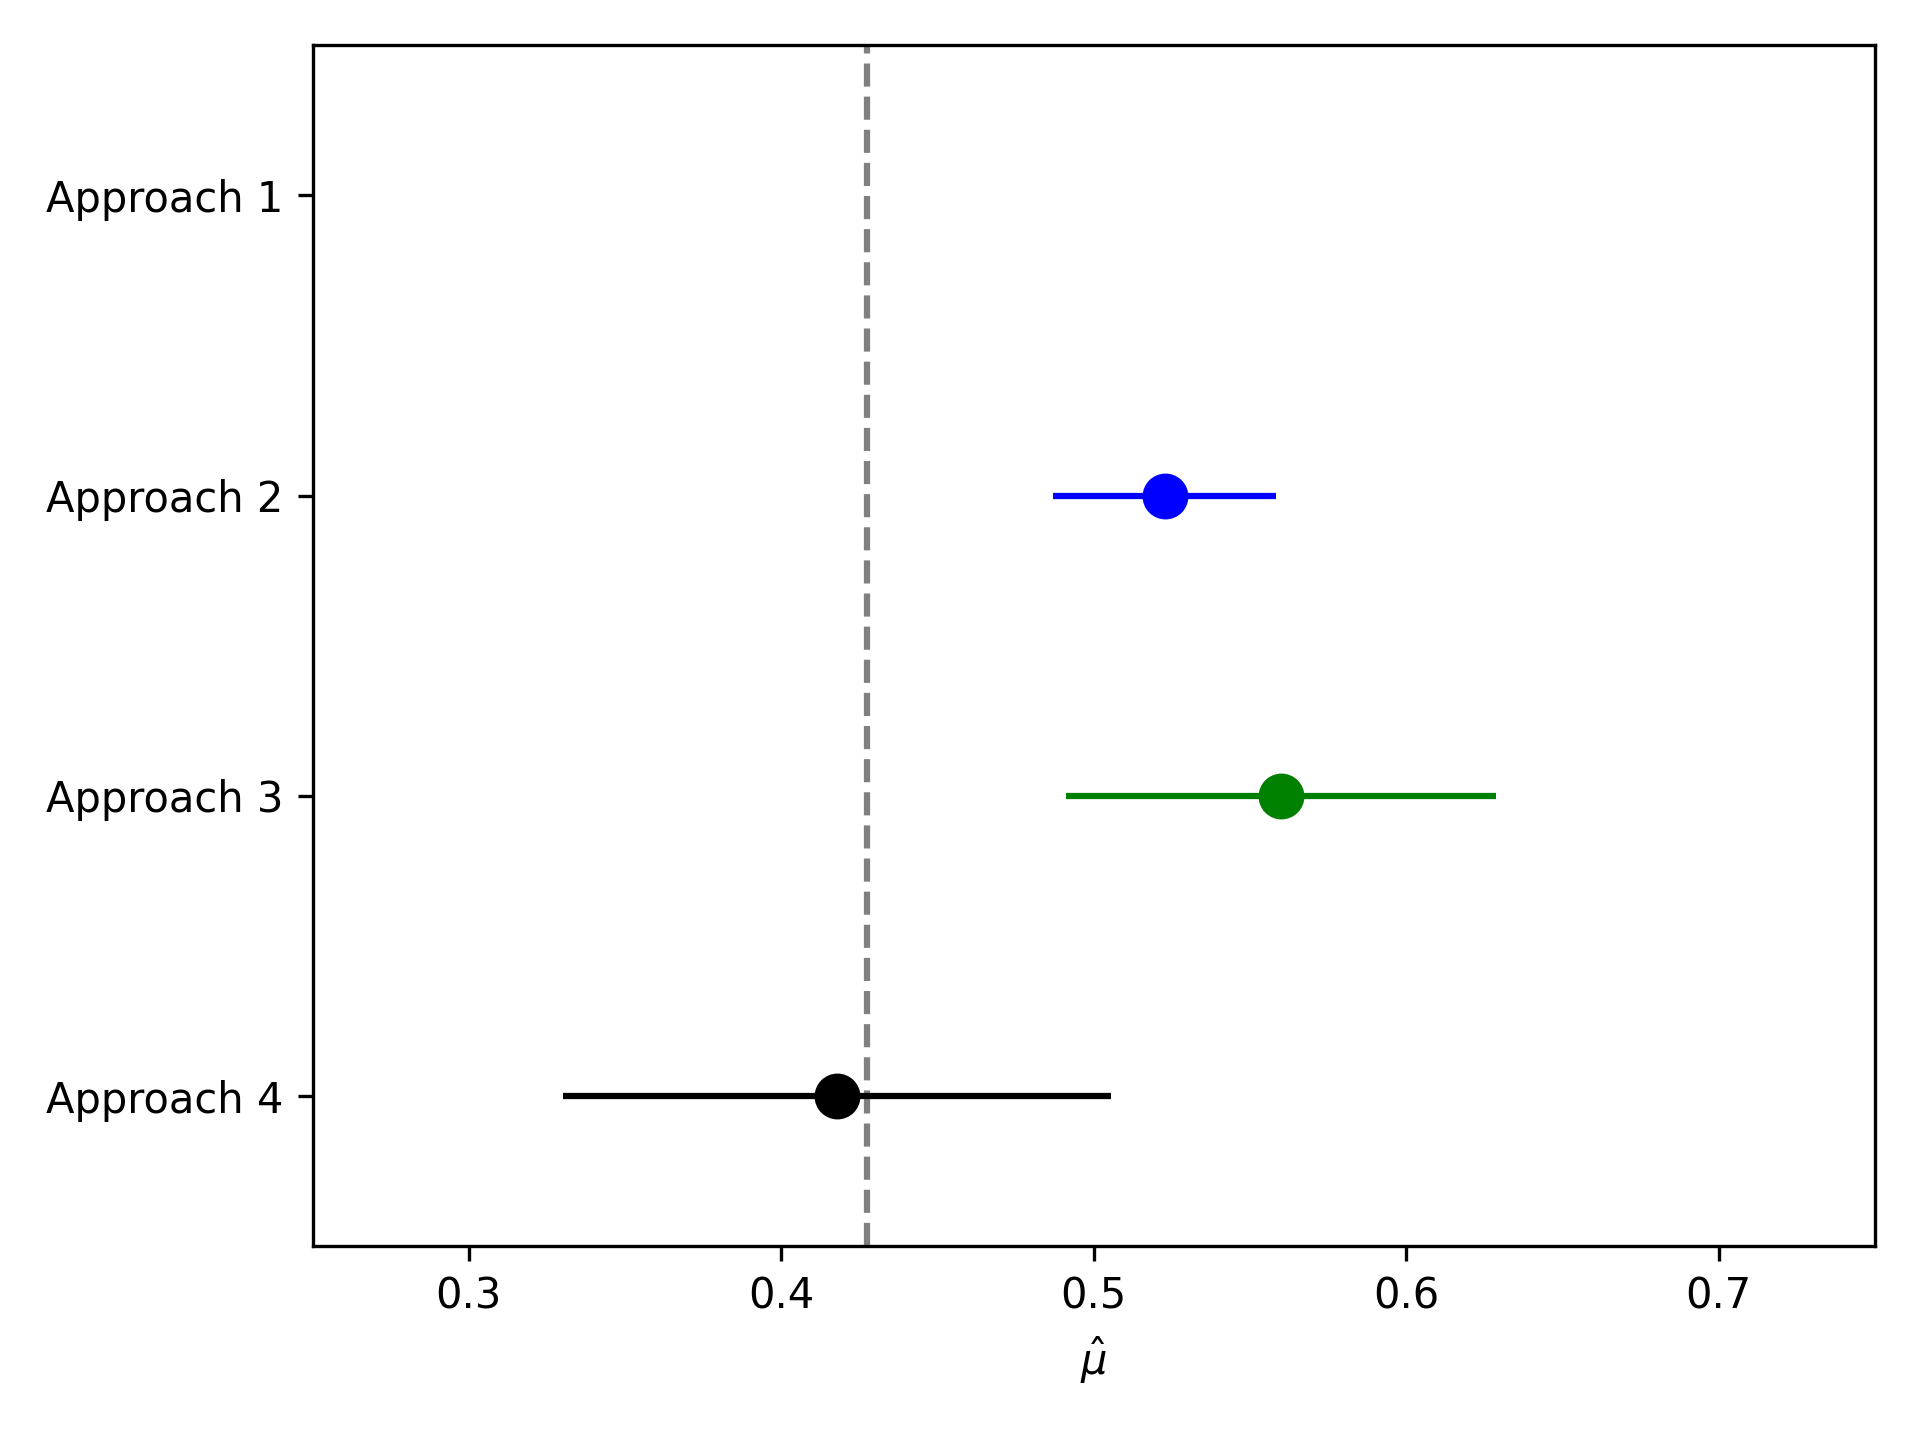
\includegraphics[scale=0.6]{code/didactic_example.png}	
\end{frame}

\section{Bridged Comparisons}

\begin{frame}{A Case Study}
	What is the risk difference at one-year of follow-up for AIDS, death, or more than a 50\% decline in CD4 count if everyone had been assigned \blue{triple} ART versus \red{mono} ART?
	\\~\\
	Data sources:
	\begin{itemize}
		\item ACTG 320
		\begin{itemize}
			\item Randomized trial comparing \blue{triple} to \violet{dual} ART
		\end{itemize}
		\item ACTG 175
		\begin{itemize}
			\item Randomized trial comparing \violet{dual} to \red{mono} ART
		\end{itemize}
	\end{itemize}~\\
	Target population: ACTG 320
\end{frame}

\begin{frame}{Default Approach}
	Transitive Comparison
	\begin{equation}
		\nonumber
		\begin{split}
			\text{\blue{Triple}} & > \text{\violet{Dual}} \\
			\text{\violet{Dual}} & > \text{\red{Mono}} \\
			% \mathclap{\rule{2cm}{0.4pt}} \\
			\therefore \text{\blue{Triple}} & > \text{\red{Mono}}
		\end{split}
	\end{equation}
	\begin{itemize}
		\item Appealing argument
		\begin{itemize}
			\item Fundamentally underlies many comparisons
		\end{itemize}
		\item Often left implicit
		\begin{itemize}
			\item Example: FDA approval following non-inferiority trial
		\end{itemize}
		\item Formalization
		\begin{itemize}
			\item Network meta-analysis, counterfactual placebos
		\end{itemize}
	\end{itemize}	
\end{frame}

\begin{frame}{Problem with Transitive Comparisons}
	Assumes "similar" target populations
	\begin{itemize}
		\item Marginal exchangeability between populations
	\end{itemize}~\\
	Highly suspect assumption
	\begin{itemize}
		\item Sample from different populations
		\item Define endpoints differently 
		\item Different rates of loss to follow-up or adherence
	\end{itemize}~\\
	How can we relax this assumption?
\end{frame}

\begin{frame}{Notation}
	$A_i=\{\red{1},\violet{2},\blue{3}\}$: ART regimens\\~\\
	
	$T_i^a$: potential time of the event under treatment $a$\\
	$T_i$: time of the event under assigned $A_i$\\
	$C_i$: time of censoring\\
	$T_i^*=\min(T_i,C_i)$,	$\;\;\;\;\delta_i = I(T_i = T_i^*)$\\~\\
	
	$W_i$: set of baseline covariates\\
	$V_i$: distinct set of baseline covariates\\
	$S_i$: population membership, $\{0,1\}$\\~\\
	
	$F_s^a(t) = \Pr(T^a < t | S=s)$
\end{frame}

\begin{frame}{Bridged Treatment Comparisons}
	Make the indirect comparisons explicit via fusion\footnote[frame]{See Breskin et al. (2021) \textit{SIM} for details}\\
	\begin{center}
		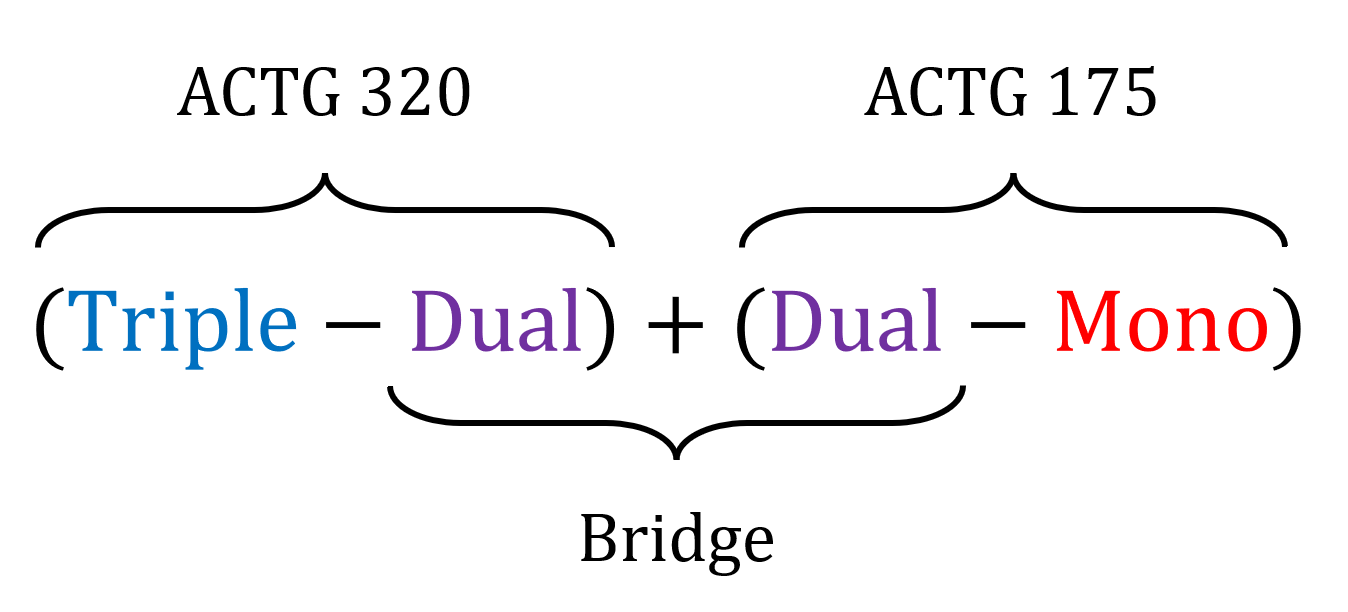
\includegraphics[scale=0.2]{images/bridge_actg.png}
	\end{center}
	Estimand
	\begin{equation} 
		\nonumber
		\begin{split}
			\psi(t) \; & = F_1^{\blue{3}}(t) - F_1^{\red{1}}(t) \\
				 % & \\
				 & = F_1^{\blue{3}}(t) - F_1^{\red{1}}(t) + \left(F_1^{\violet{2}}(t) - F_1^{\violet{2}}(t)\right) \\
				 & = \left(F_1^{\blue{3}}(t) - F_1^{\violet{2}}(t)\right) + \left(F_1^{\violet{2}}(t) - F_1^{\red{1}}(t)\right)
		\end{split}
	\end{equation}
\end{frame}

\begin{frame}{Identification: \blue{Triple} vs \violet{Dual}}
	\[F_1^{\blue{3}}(t) - F_1^{\violet{2}}(t)\]~\\
	Treatment	
	\[T_i = T_i^a \text{ for } a = A_i\]
	\[\Pr(T^a < t | S = 1) = \Pr(T^a < t |A=a, S=1) \text{ for } a \in \{2, 3\}\]
	\[\Pr(A = a | S=1) > 0 \text{ for } a \in \{2, 3\}\]
	Censoring
	\[\Pr(T < t |A,W,S=1) = \Pr(T < t |C>t,A,W,S=1)\]
	\[\Pr(C > T | A=a,W=w,S=1) > 0 \; \forall \; \Pr(A=a,W=w | S=1) > 0\]
\end{frame}

\begin{frame}{Estimation: \blue{Triple} vs \violet{Dual}}
	Inverse probability weighting estimator\footnote[frame]{Identification implies estimation hereafter following stability from parametric or semiparametric restrictions. Estimation also requires correct model specification}
	\[\hat{F}_{320}^{a}(t) = n_{320}^{-1} \sum_{i=1}^{n} \frac{I(A_i = a) I(S_i = 1) I(T_i^* \le t) \delta_i}{\Pr(A_i = a |S_i = 1) \pi_C(W_i, A_i, S_i; \hat{\alpha})}\]~\\
	for $a \in \{\violet{2}, \blue{3}\}$, where 
	\[n_{320} = \sum_{i=1}^{n} I(S_i = 1)\]
	\[\pi_C(W_i, A_i, S_i; \hat{\alpha}) = \Pr(C_i>t | W_i, A_i, S_i; \hat{\alpha}) \]
\end{frame}

\begin{frame}{Identification: \violet{Dual} vs \red{Mono}}
	\[F_1^{\violet{2}}(t) - F_1^{\red{1}}(t)\]~\\
	Similar identification assumption for treatment and censoring
	\begin{itemize}
		\item Unwilling to assume trials are random samples of same population
	\end{itemize}~\\
	Transport\footnote[frame]{Simple transitivity arguments are the special case where $V=\emptyset$}
	\[\Pr(T^a < t | V, S = 1) = \Pr(T^a < t | V, S=0)\]
	\[\Pr(S=0 | V=v) > 0 \text{ for all } v \text{ where } \Pr(S=1 | V=v) > 0\]
\end{frame}

\begin{frame}{Estimation: \violet{Dual} vs \red{Mono}}
	\[\hat{F}_{175}^{a}(t) = \hat{n}_{175}^{-1} \sum_{i=1}^{n} \frac{I(A_i = a) I(S_i = 1) I(T_i^* \le t) \delta_i}{\Pr(A_i = a |S_i = 1) \pi_C(W_i, A_i, S_i; \hat{\alpha})} \times \frac{1 - \pi_S(V_i; \hat{\beta})}{\pi_S(V_i; \hat{\beta})}\]~\\
	for $a \in \{\red{1}, \violet{2}\}$, where
	\[\hat{n}_{175} = \sum_{i=1}^{n} I(S_i = 0) \frac{1 - \pi_S(V_i; \hat{\beta})}{\pi_S(V_i; \hat{\beta})}\]
	\[\pi_S(V_i; \hat{\beta}) = \Pr(S_i = 1 | V_i; \hat{\beta})\]
\end{frame}

\begin{frame}{Application to ACTG}
	Implemented in Python 3.6+\footnote[frame]{Using \texttt{NumPy}, \texttt{SciPy}, \texttt{statsmodels}}
	\\~\\
	$\pi_C(W_i, A_i, S_i; \hat{\alpha})$
	\begin{itemize}
		\item Stratified Cox PH model \& Breslow estimator
		\item Stratified by trial and ART
		\item $W$: age, gender, race, injection drug use, Karnofsky score 
	\end{itemize}~\\
	$\pi_S(V_i; \hat{\beta})$
	\begin{itemize}
		\item Logistic regression
		\item $V=W$
	\end{itemize}
\end{frame}

\begin{frame}{A Testable Implication}
	Identification strategy for $\psi$ required
	\[F_1^{\violet{2}}(t) - F_1^{\violet{2}}(t) = 0\]
	which implies
	\[E\left[\hat{F}_{320}^{\violet{2}}(t)\right] - E\left[\hat{F}_{175}^{\violet{2}}(t)\right] = 0\]
	~\\
	Therefore, can compare the shared arms
	\begin{itemize}
		\item If non-zero then at least one assumption is wrong
		\item Ways to assess
		\begin{itemize}
			\item Graphically\footnote[frame]{Twister plot as described in Zivich et al. (2021) \textit{Am J Epidemiol}}
			\item Numerically via a permutation test based on area between the risk functions
		\end{itemize}
	\end{itemize}
\end{frame}

\begin{frame}{Testable Implication: Naive}
	\centering
	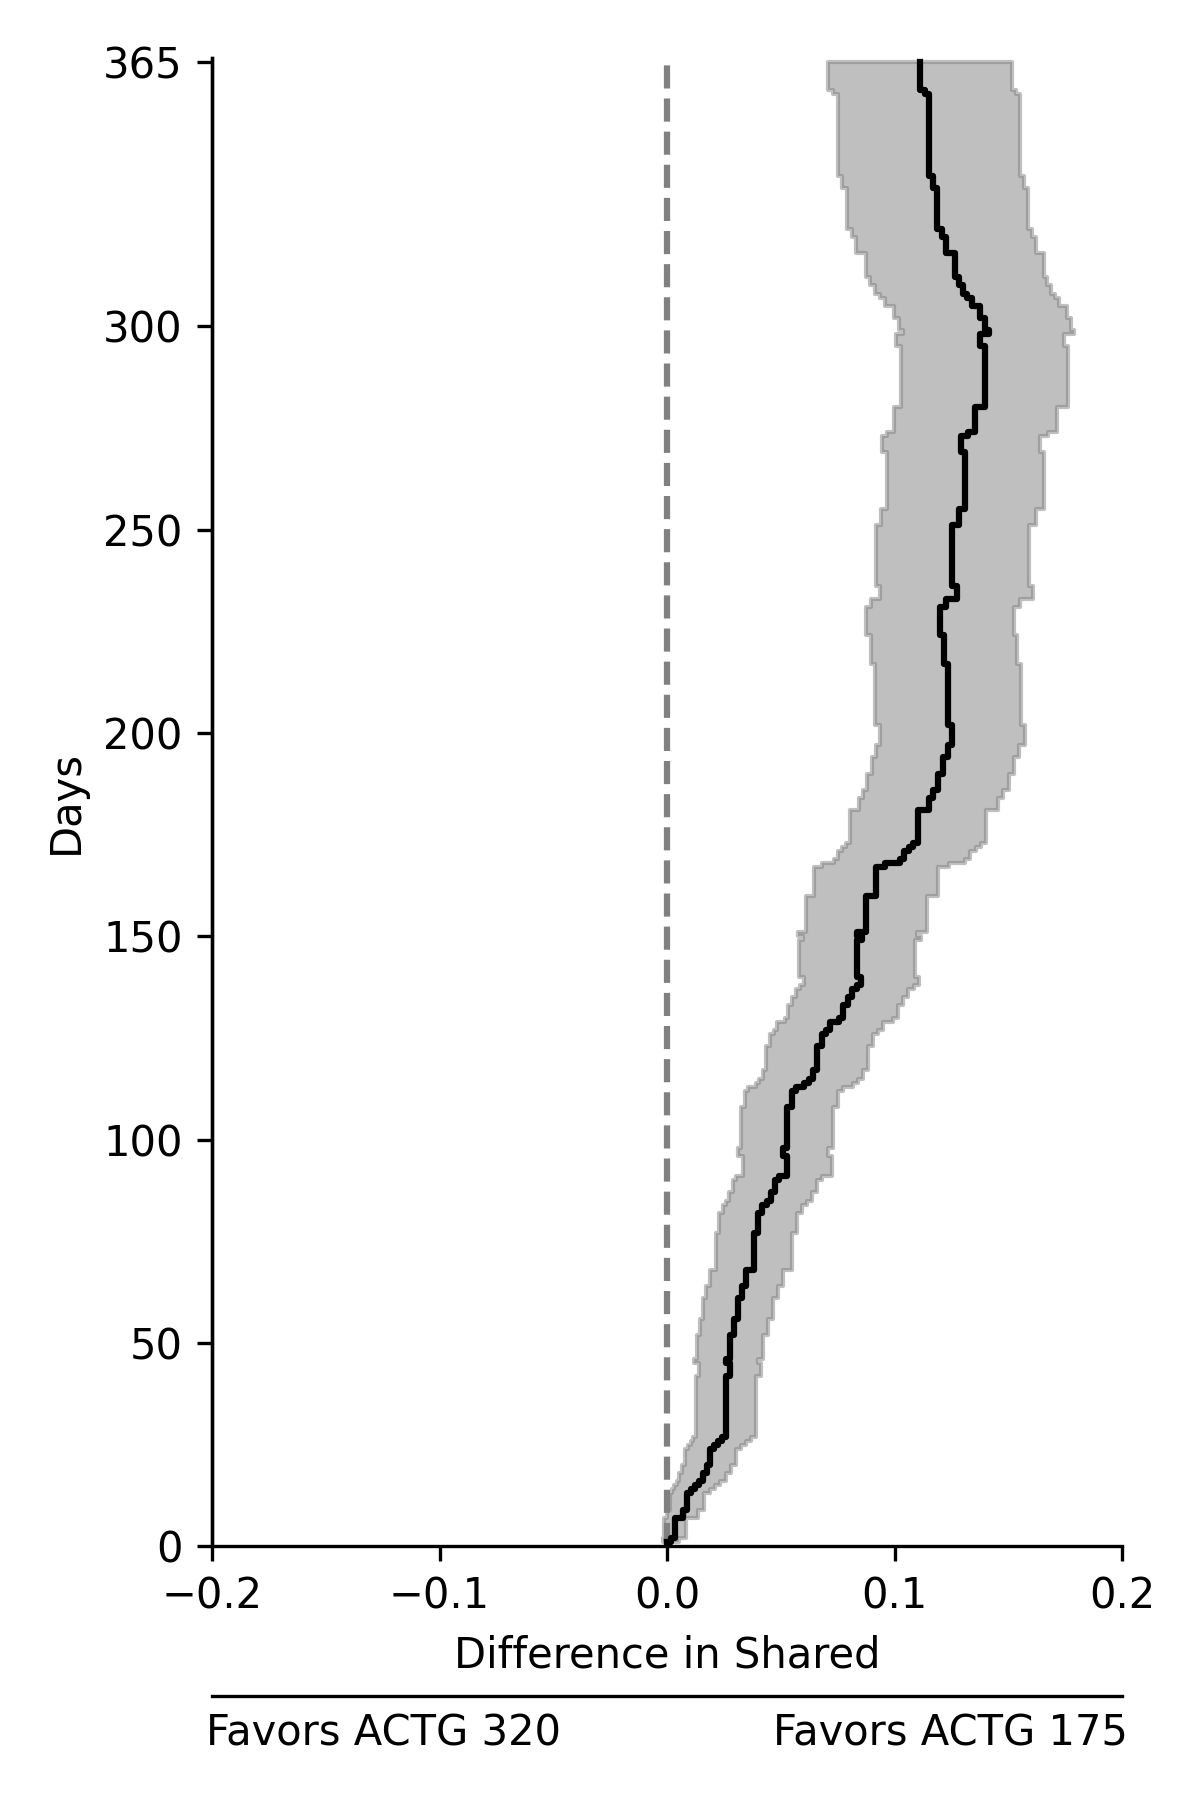
\includegraphics[scale=0.33]{images/diagnostic_graph_naive.png}	
	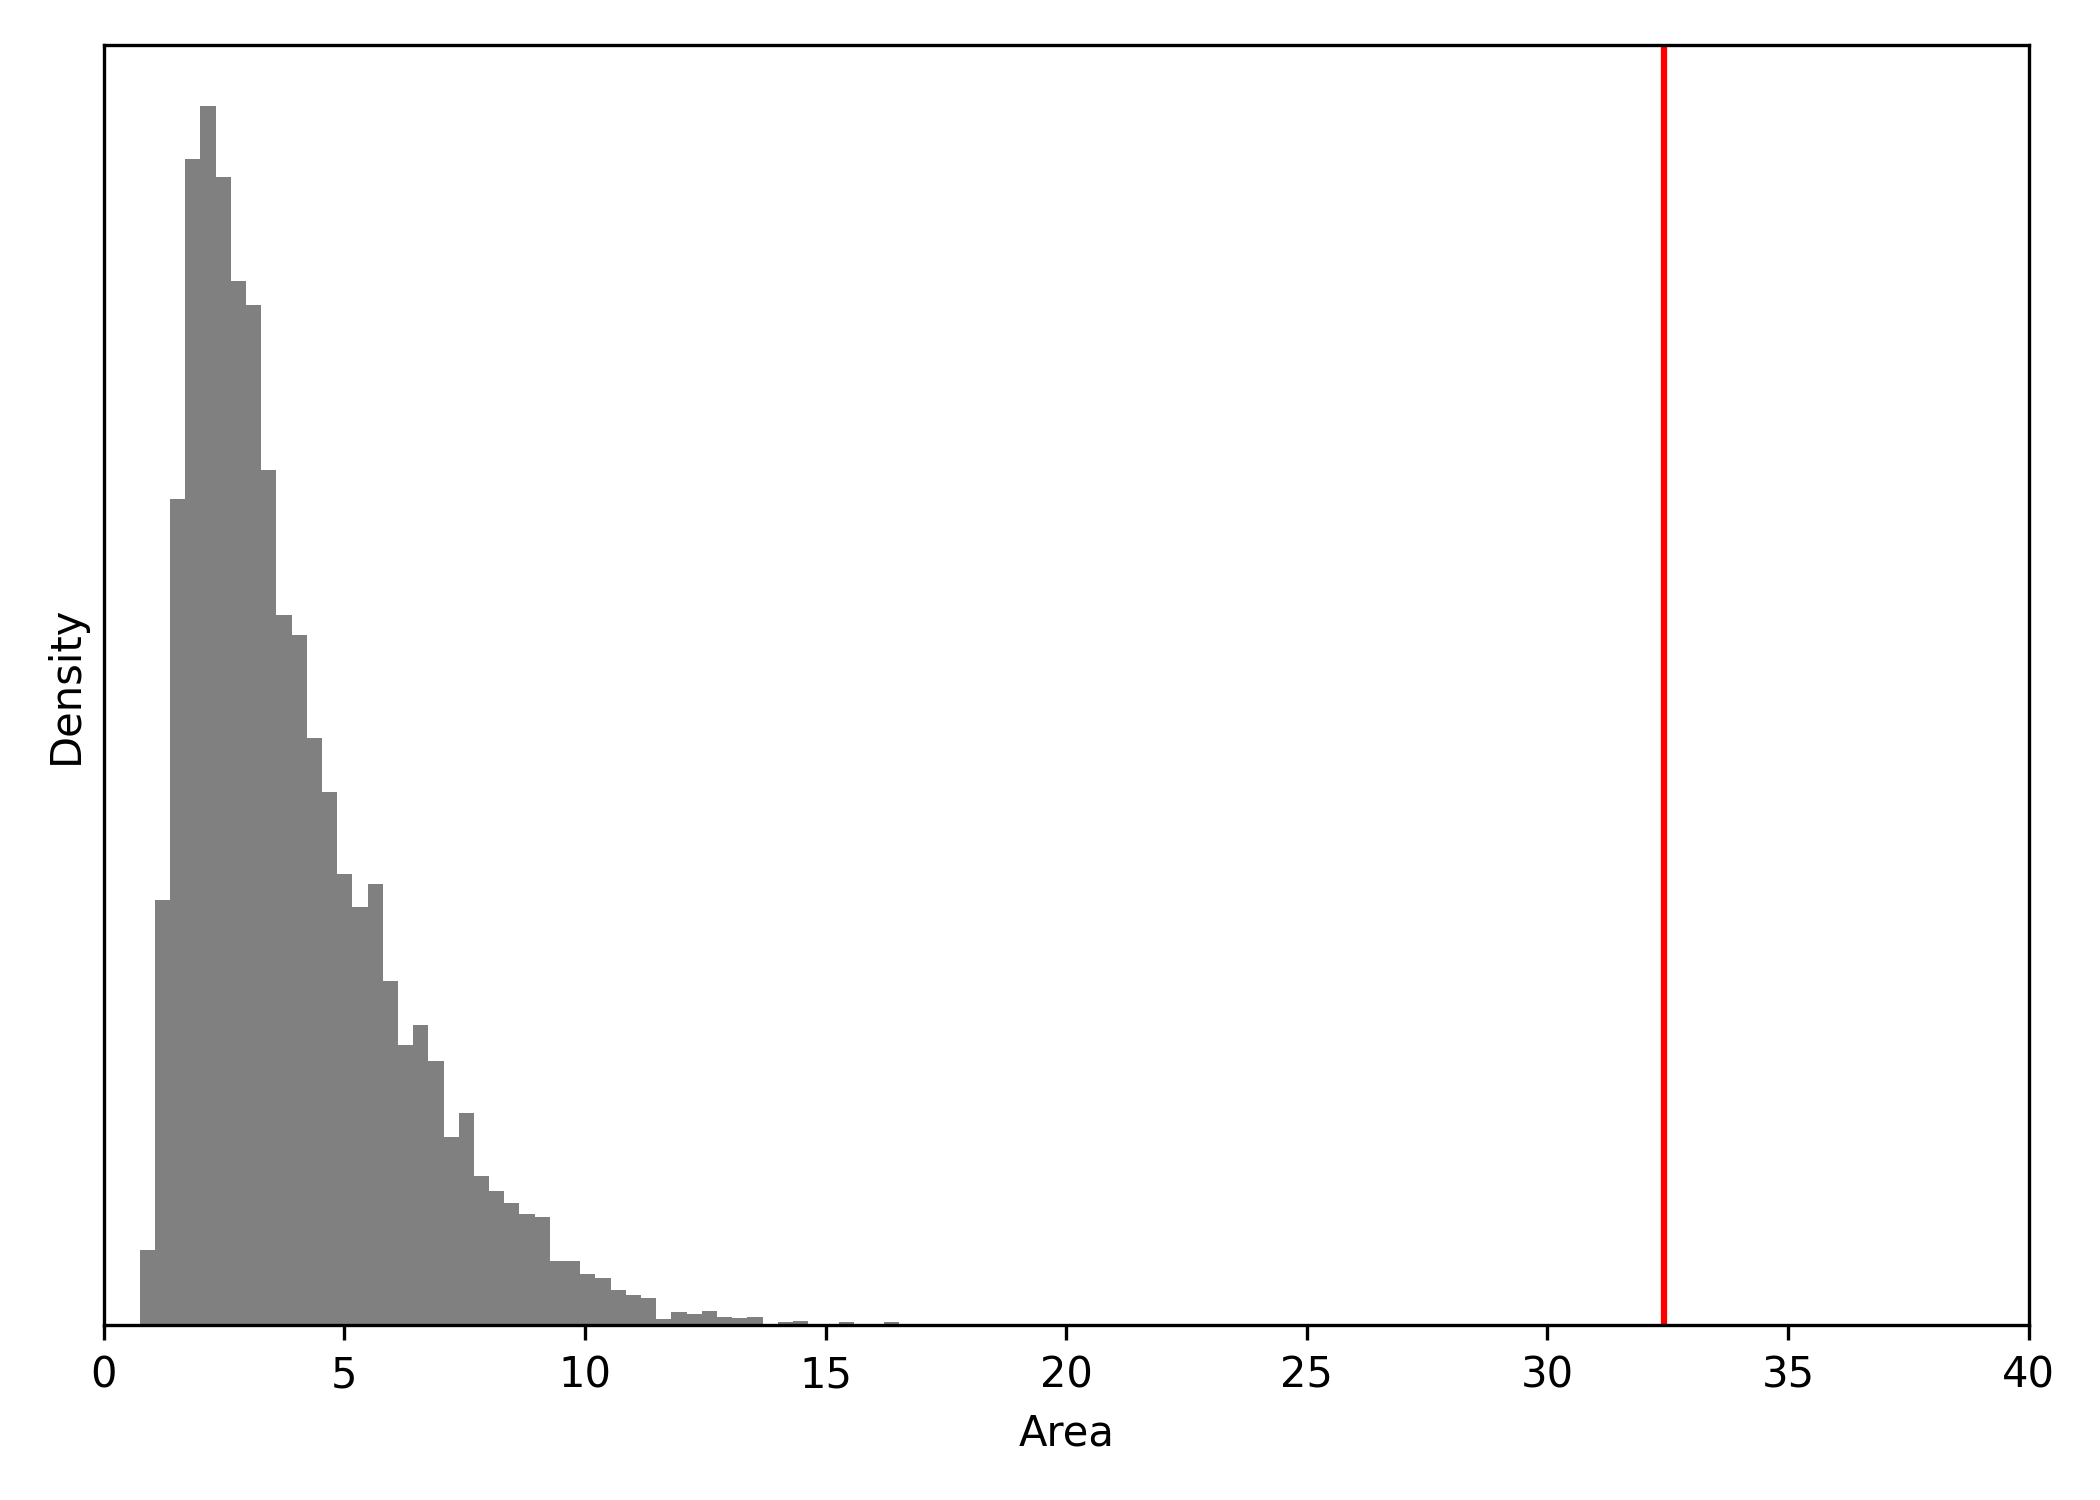
\includegraphics[scale=0.4]{images/diagnostic_test_naive.png}	
\end{frame}

\begin{frame}{Testable Implication: transported}
	\centering
	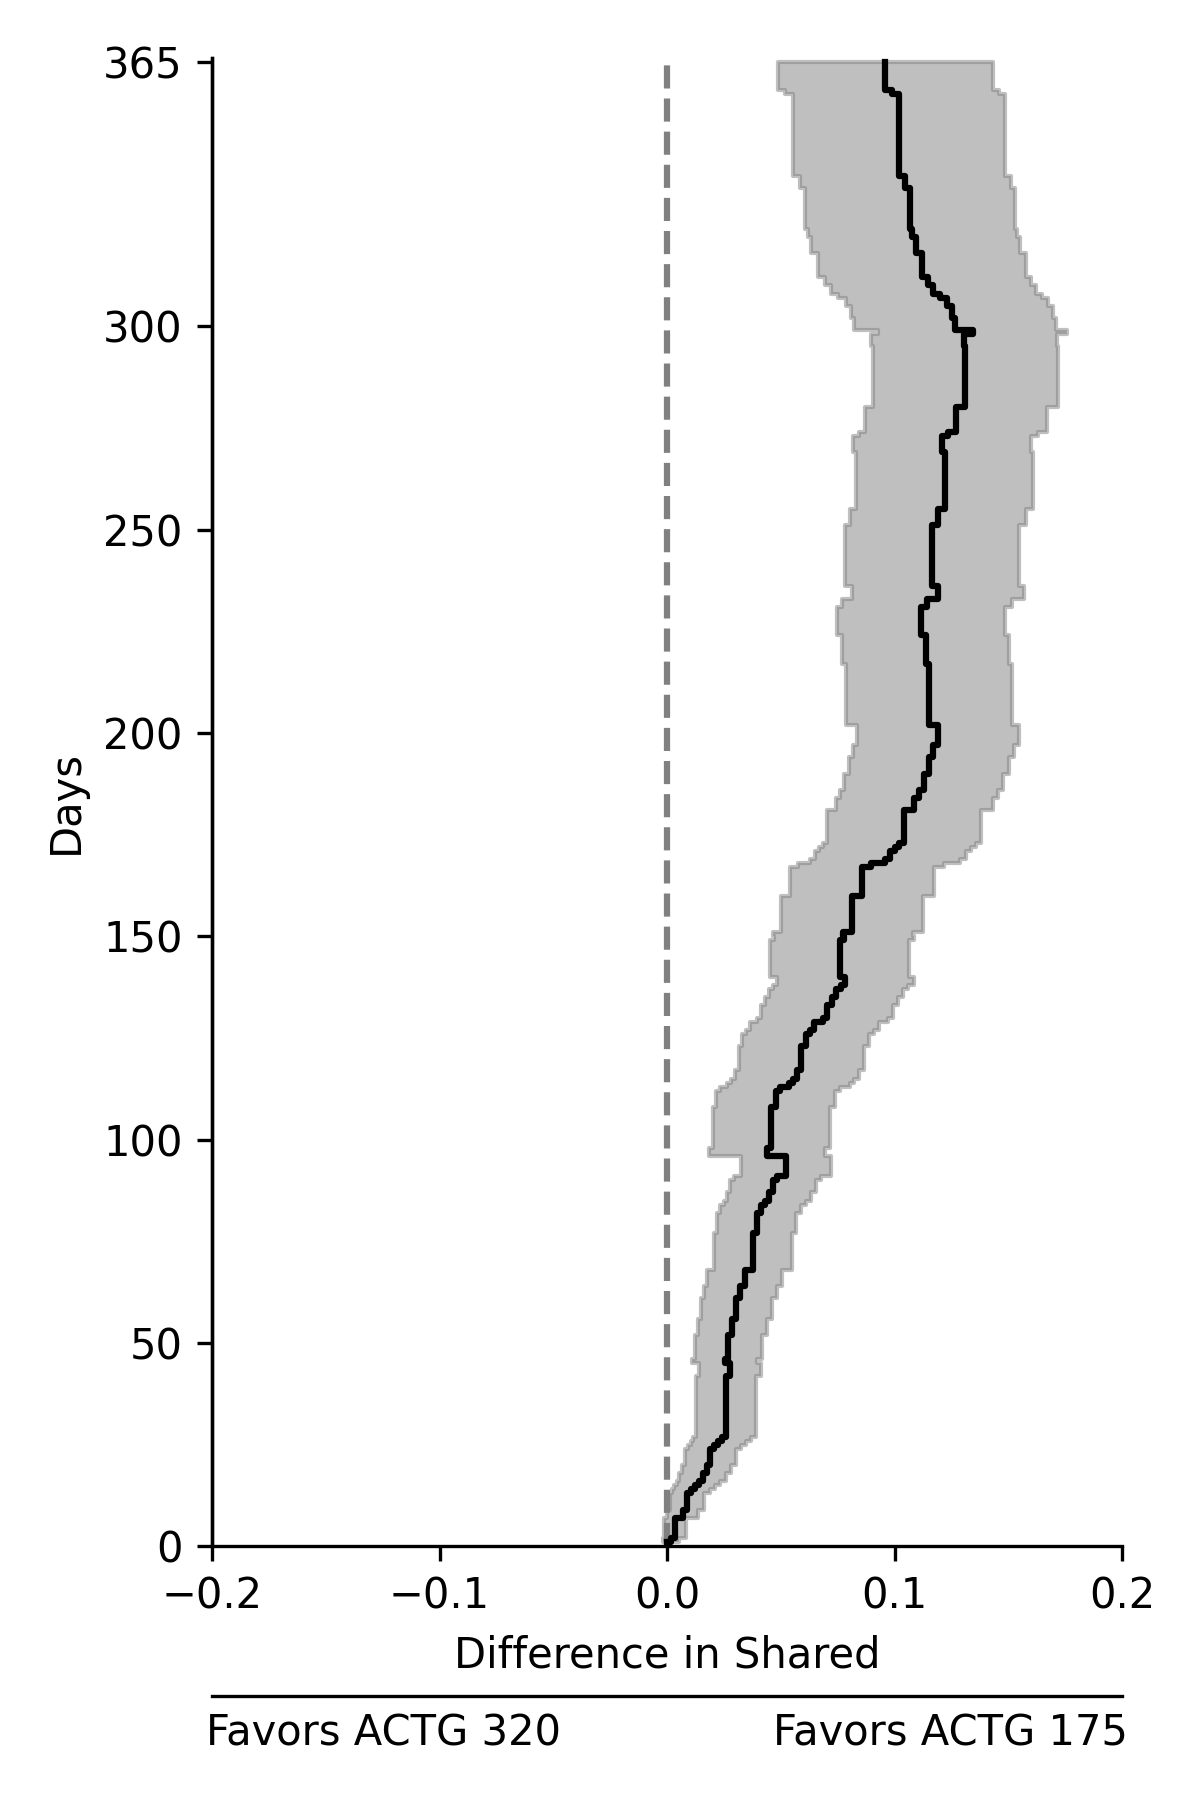
\includegraphics[scale=0.33]{images/diagnostic_graph_trn.png}	
	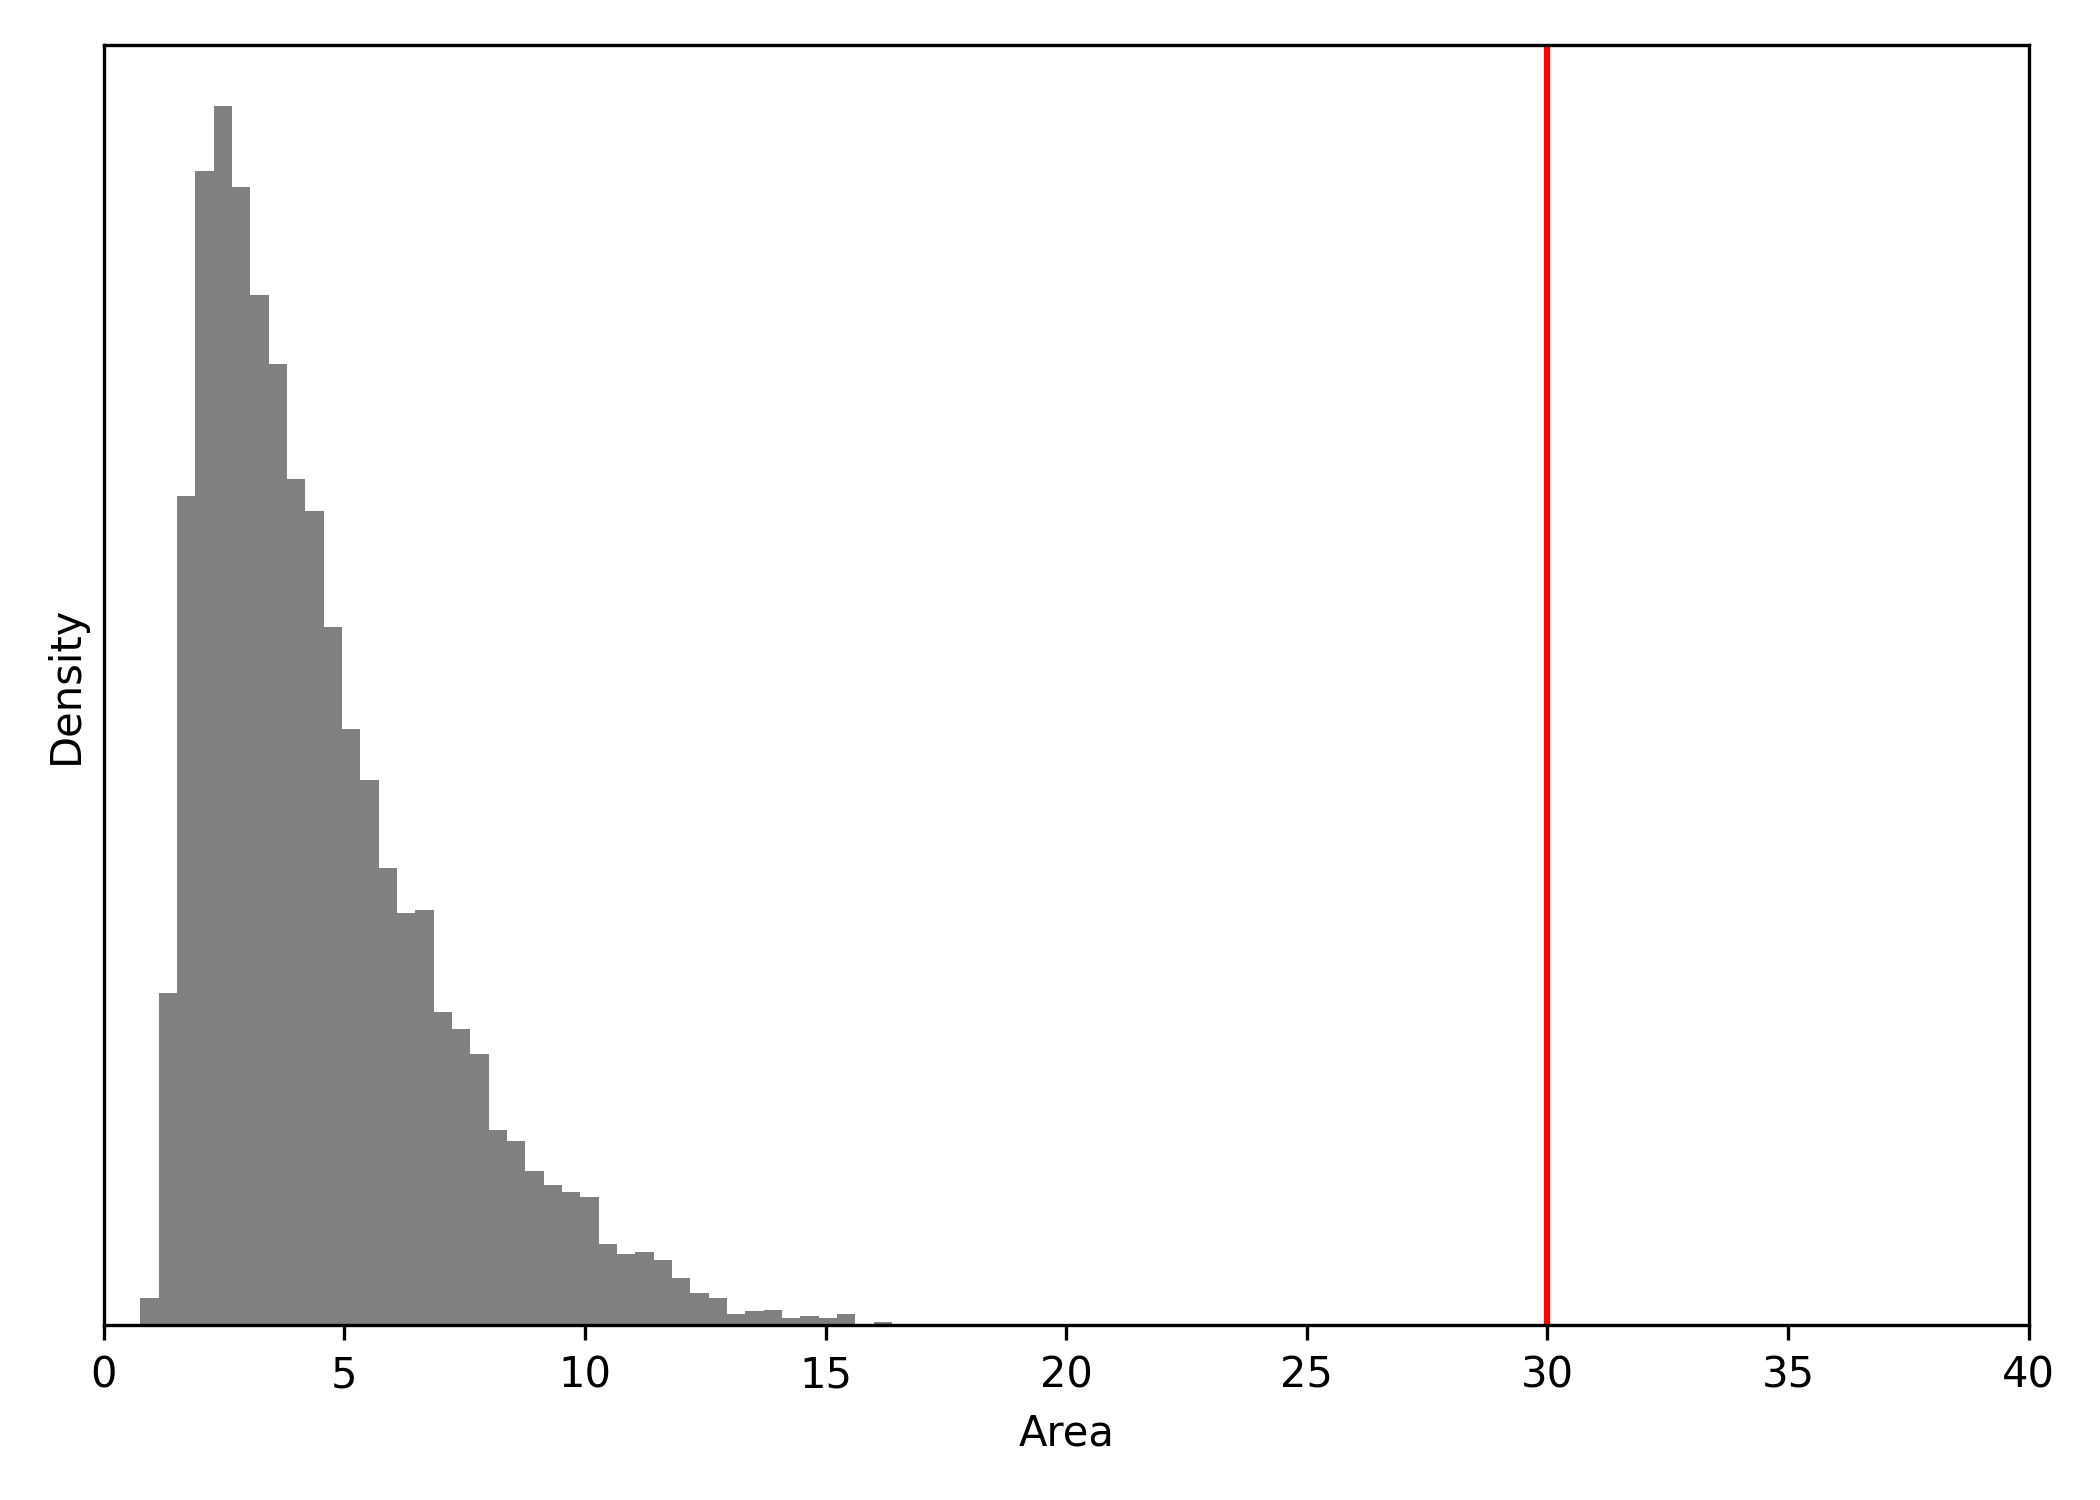
\includegraphics[scale=0.4]{images/diagnostic_test_trn.png}	
\end{frame}

\begin{frame}{The Distinction}
	\centering
	ACTG 175
	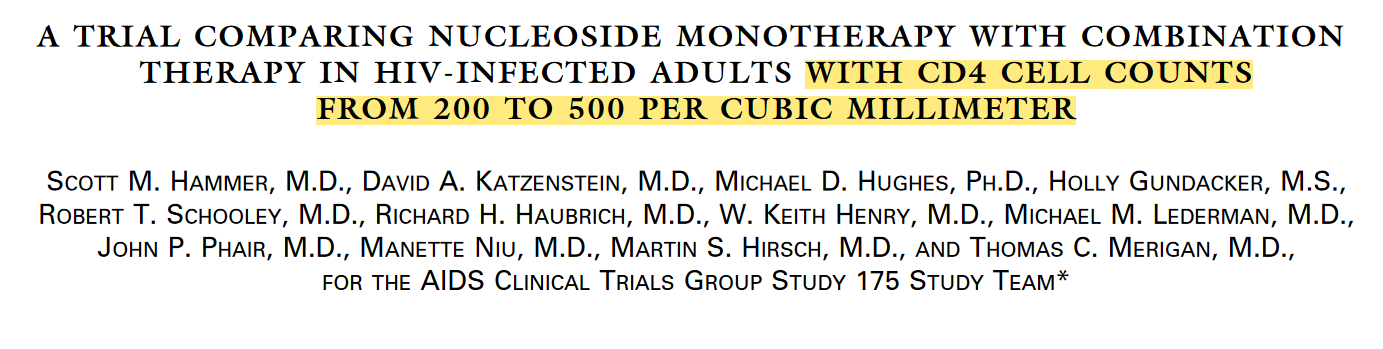
\includegraphics[scale=0.35]{images/actg175.png}\\~\\
	ACTG 320
	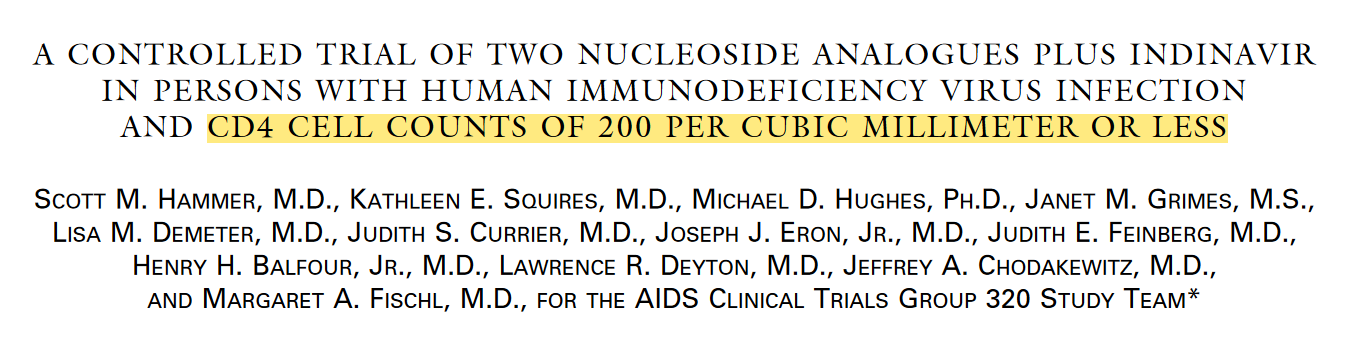
\includegraphics[scale=0.35]{images/actg320.png}
\end{frame}

\begin{frame}{Baseline CD4 counts}
	\centering
	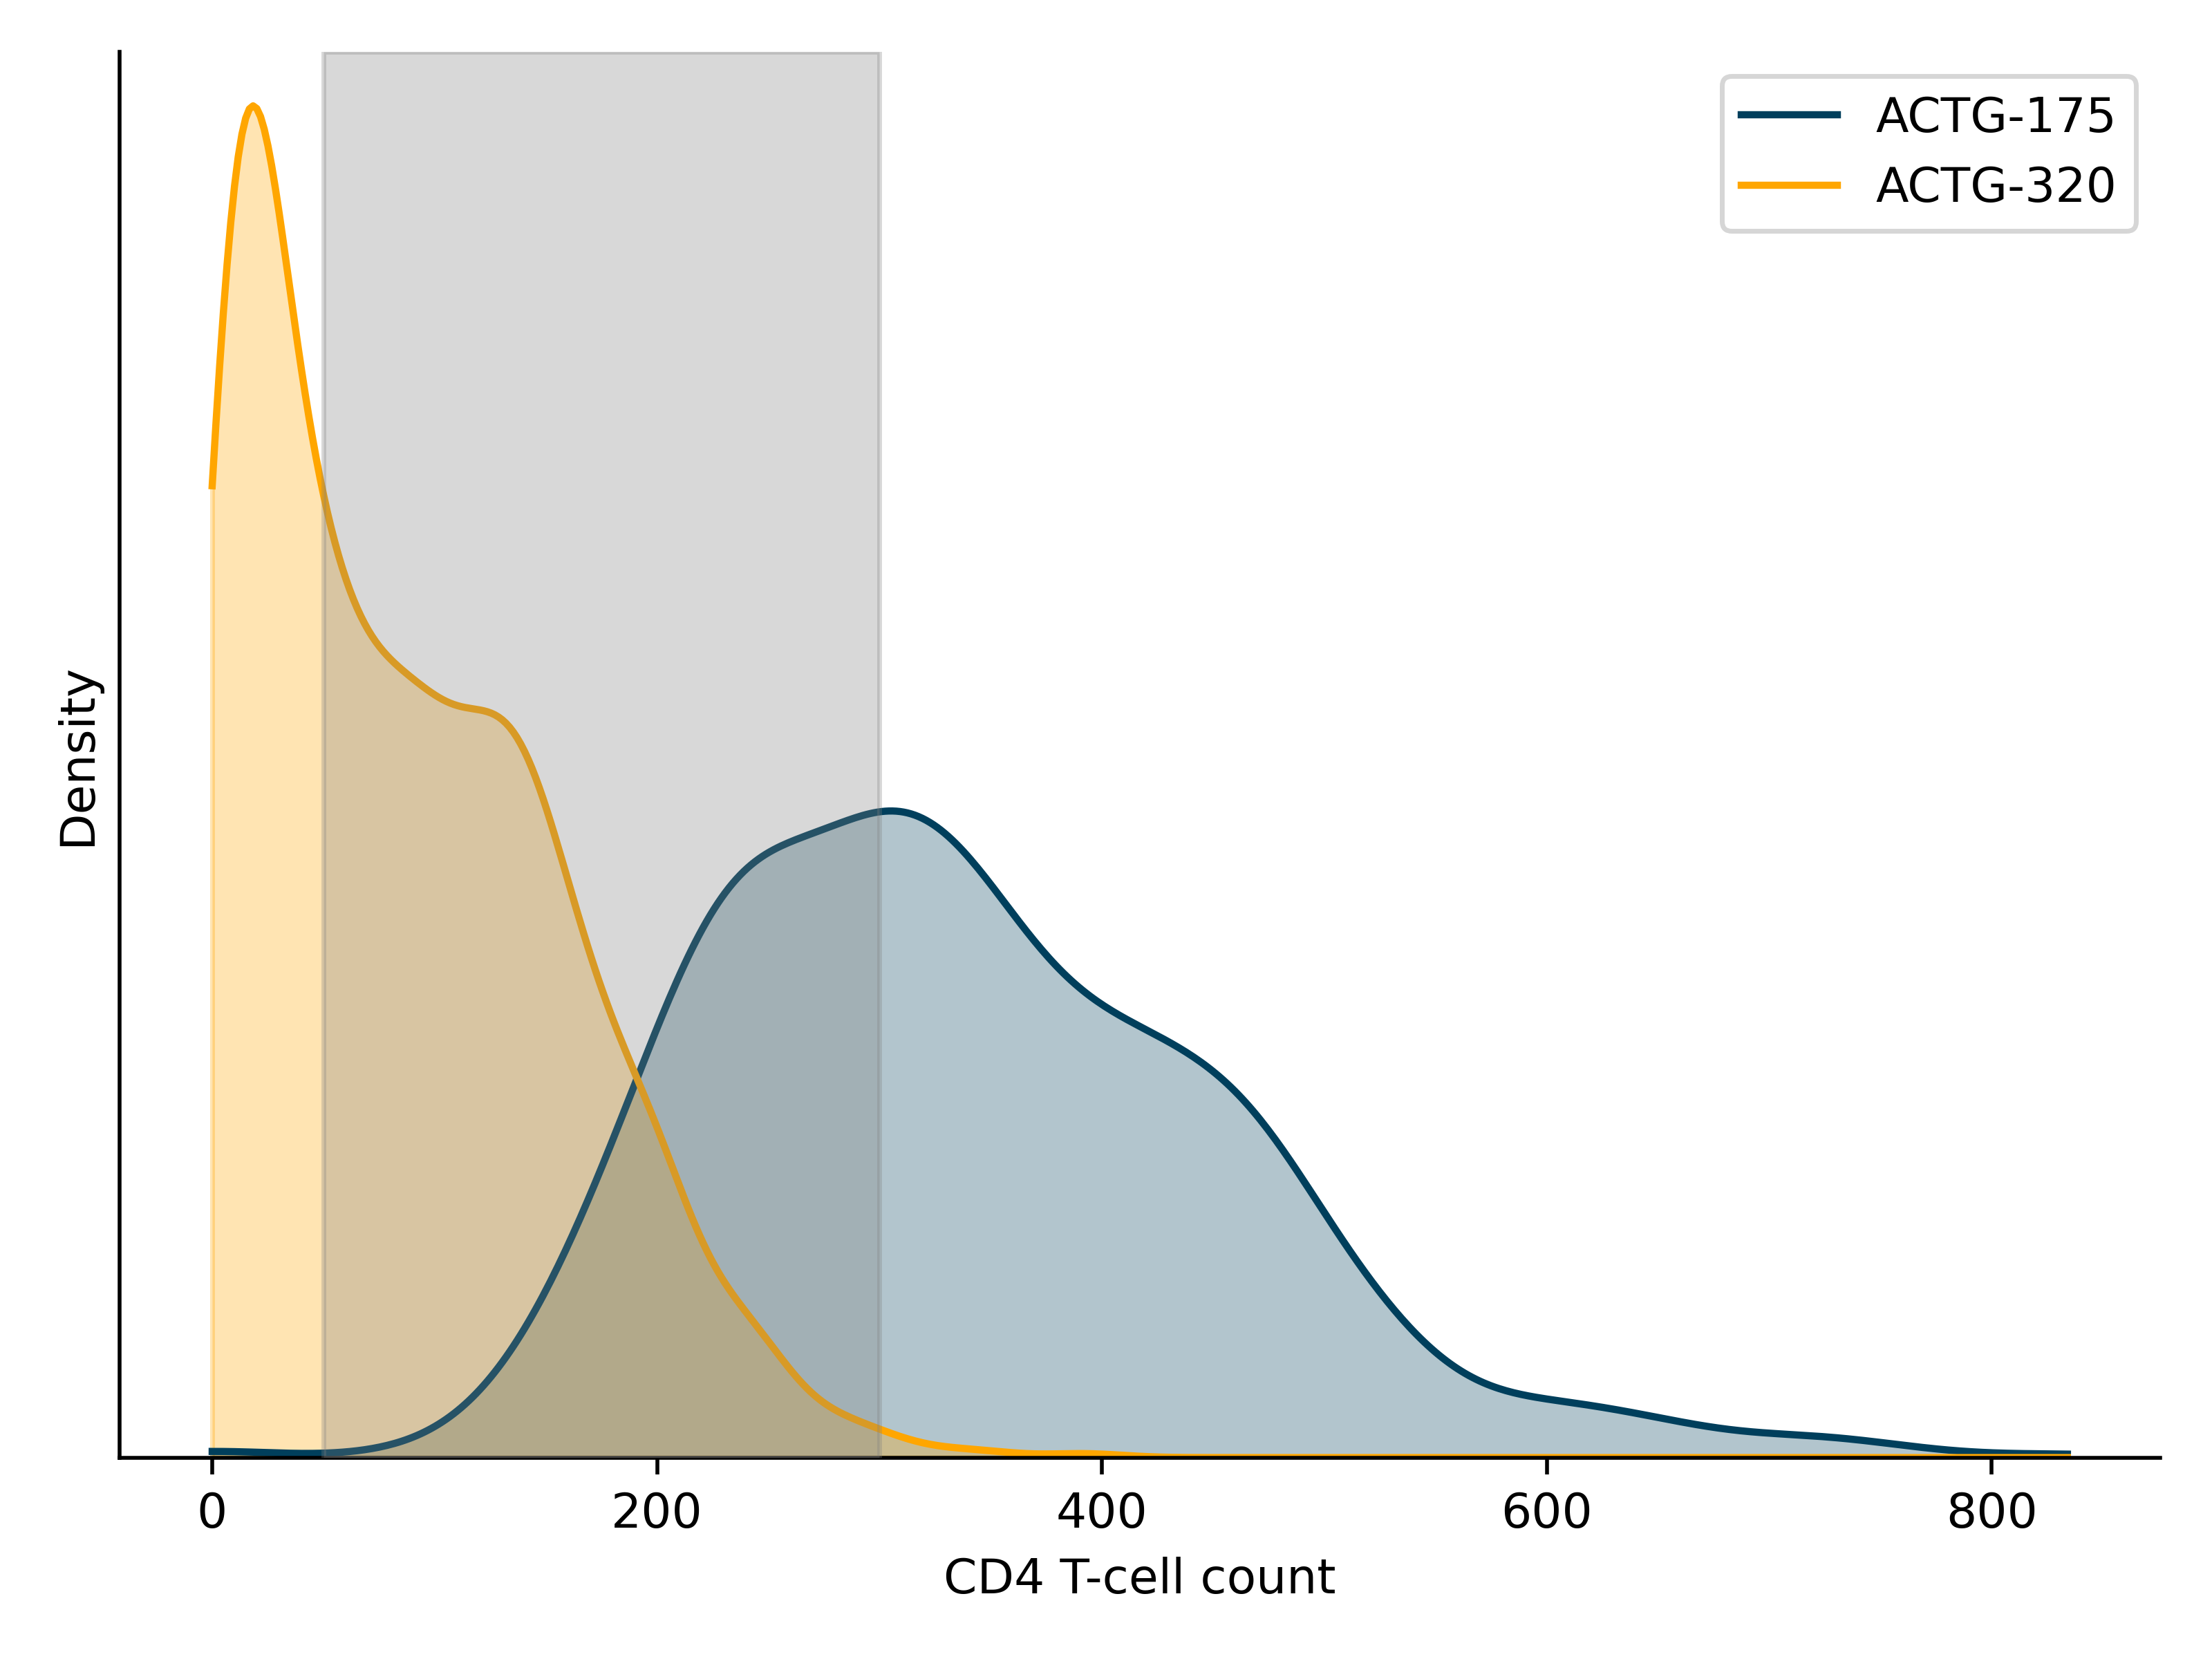
\includegraphics[scale=0.5]{images/cd4_by_study.png}	
\end{frame}

\begin{frame}{Testable Implication: transported and CD4 restricted}
	\centering
	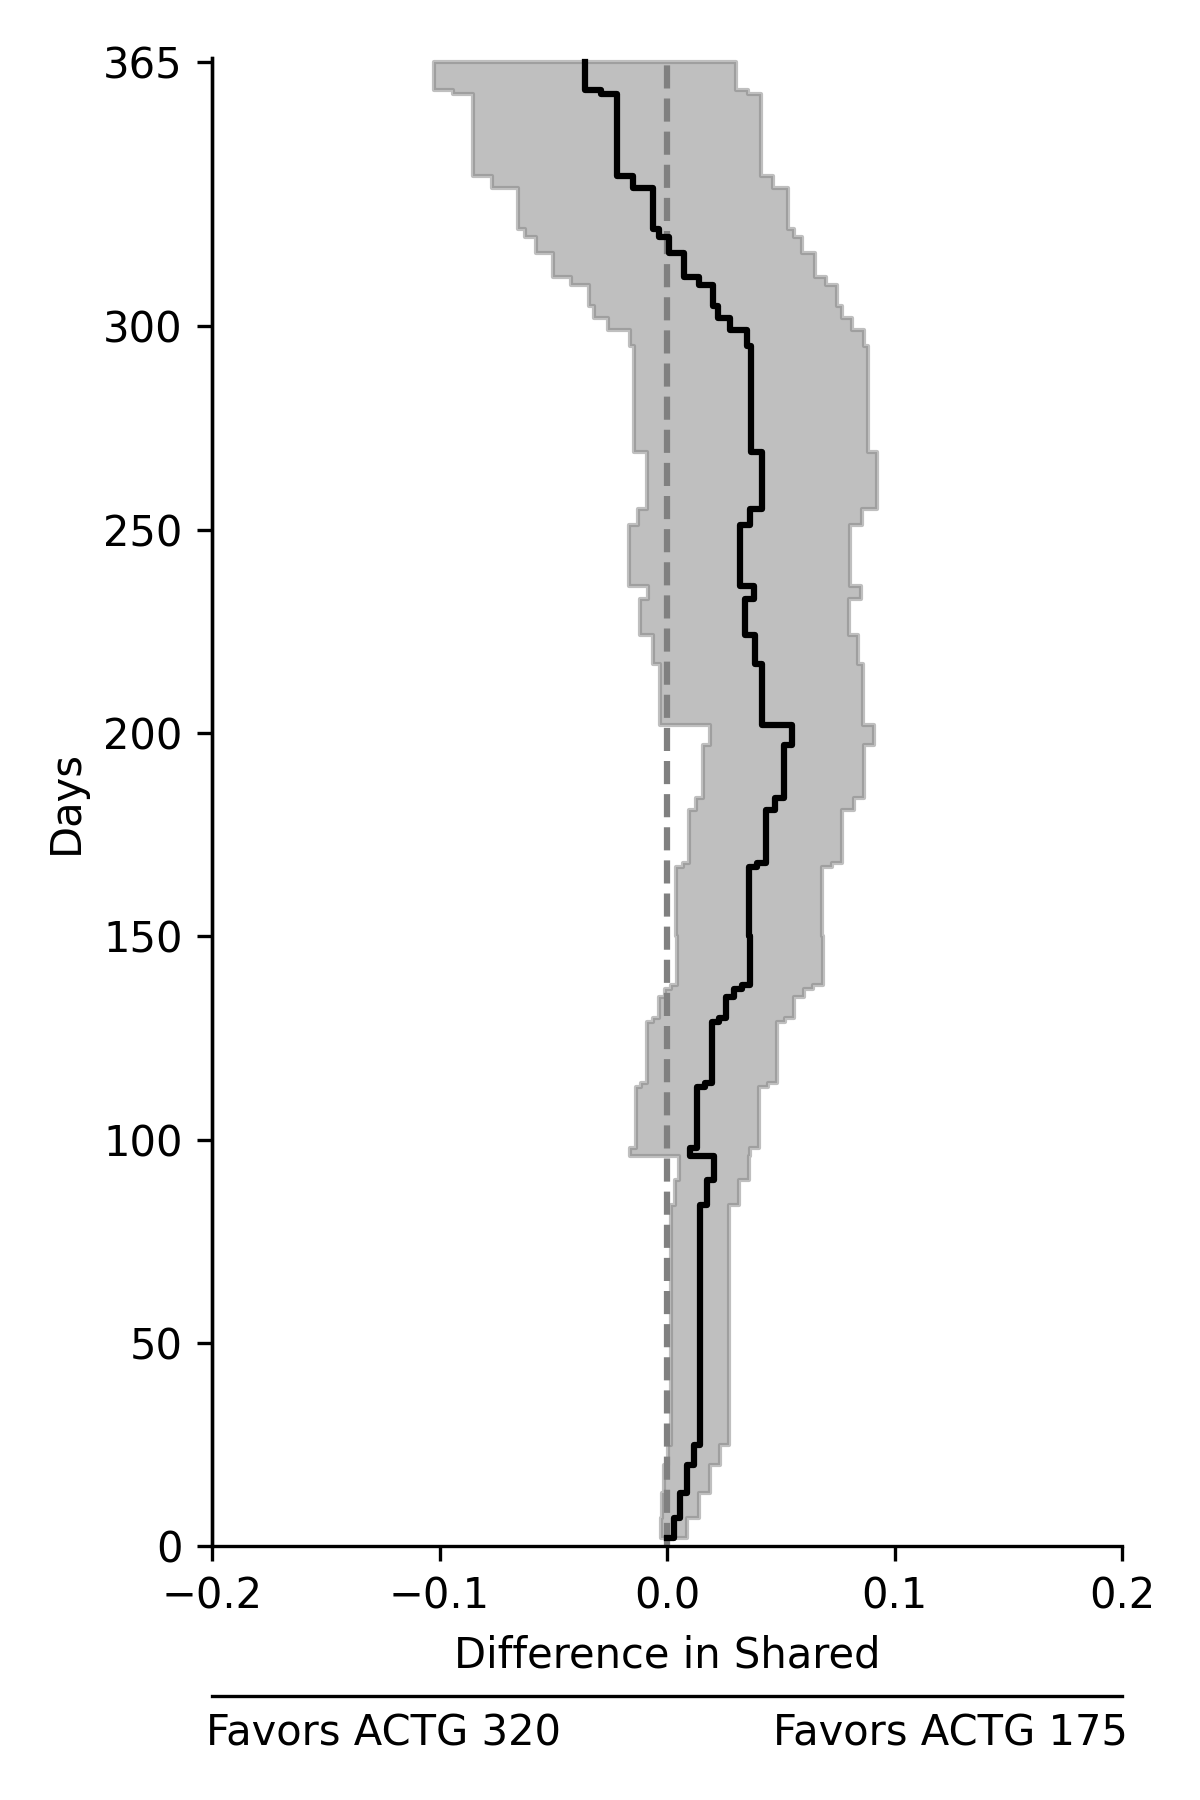
\includegraphics[scale=0.33]{images/diagnostic_graph_rtrn.png}	
	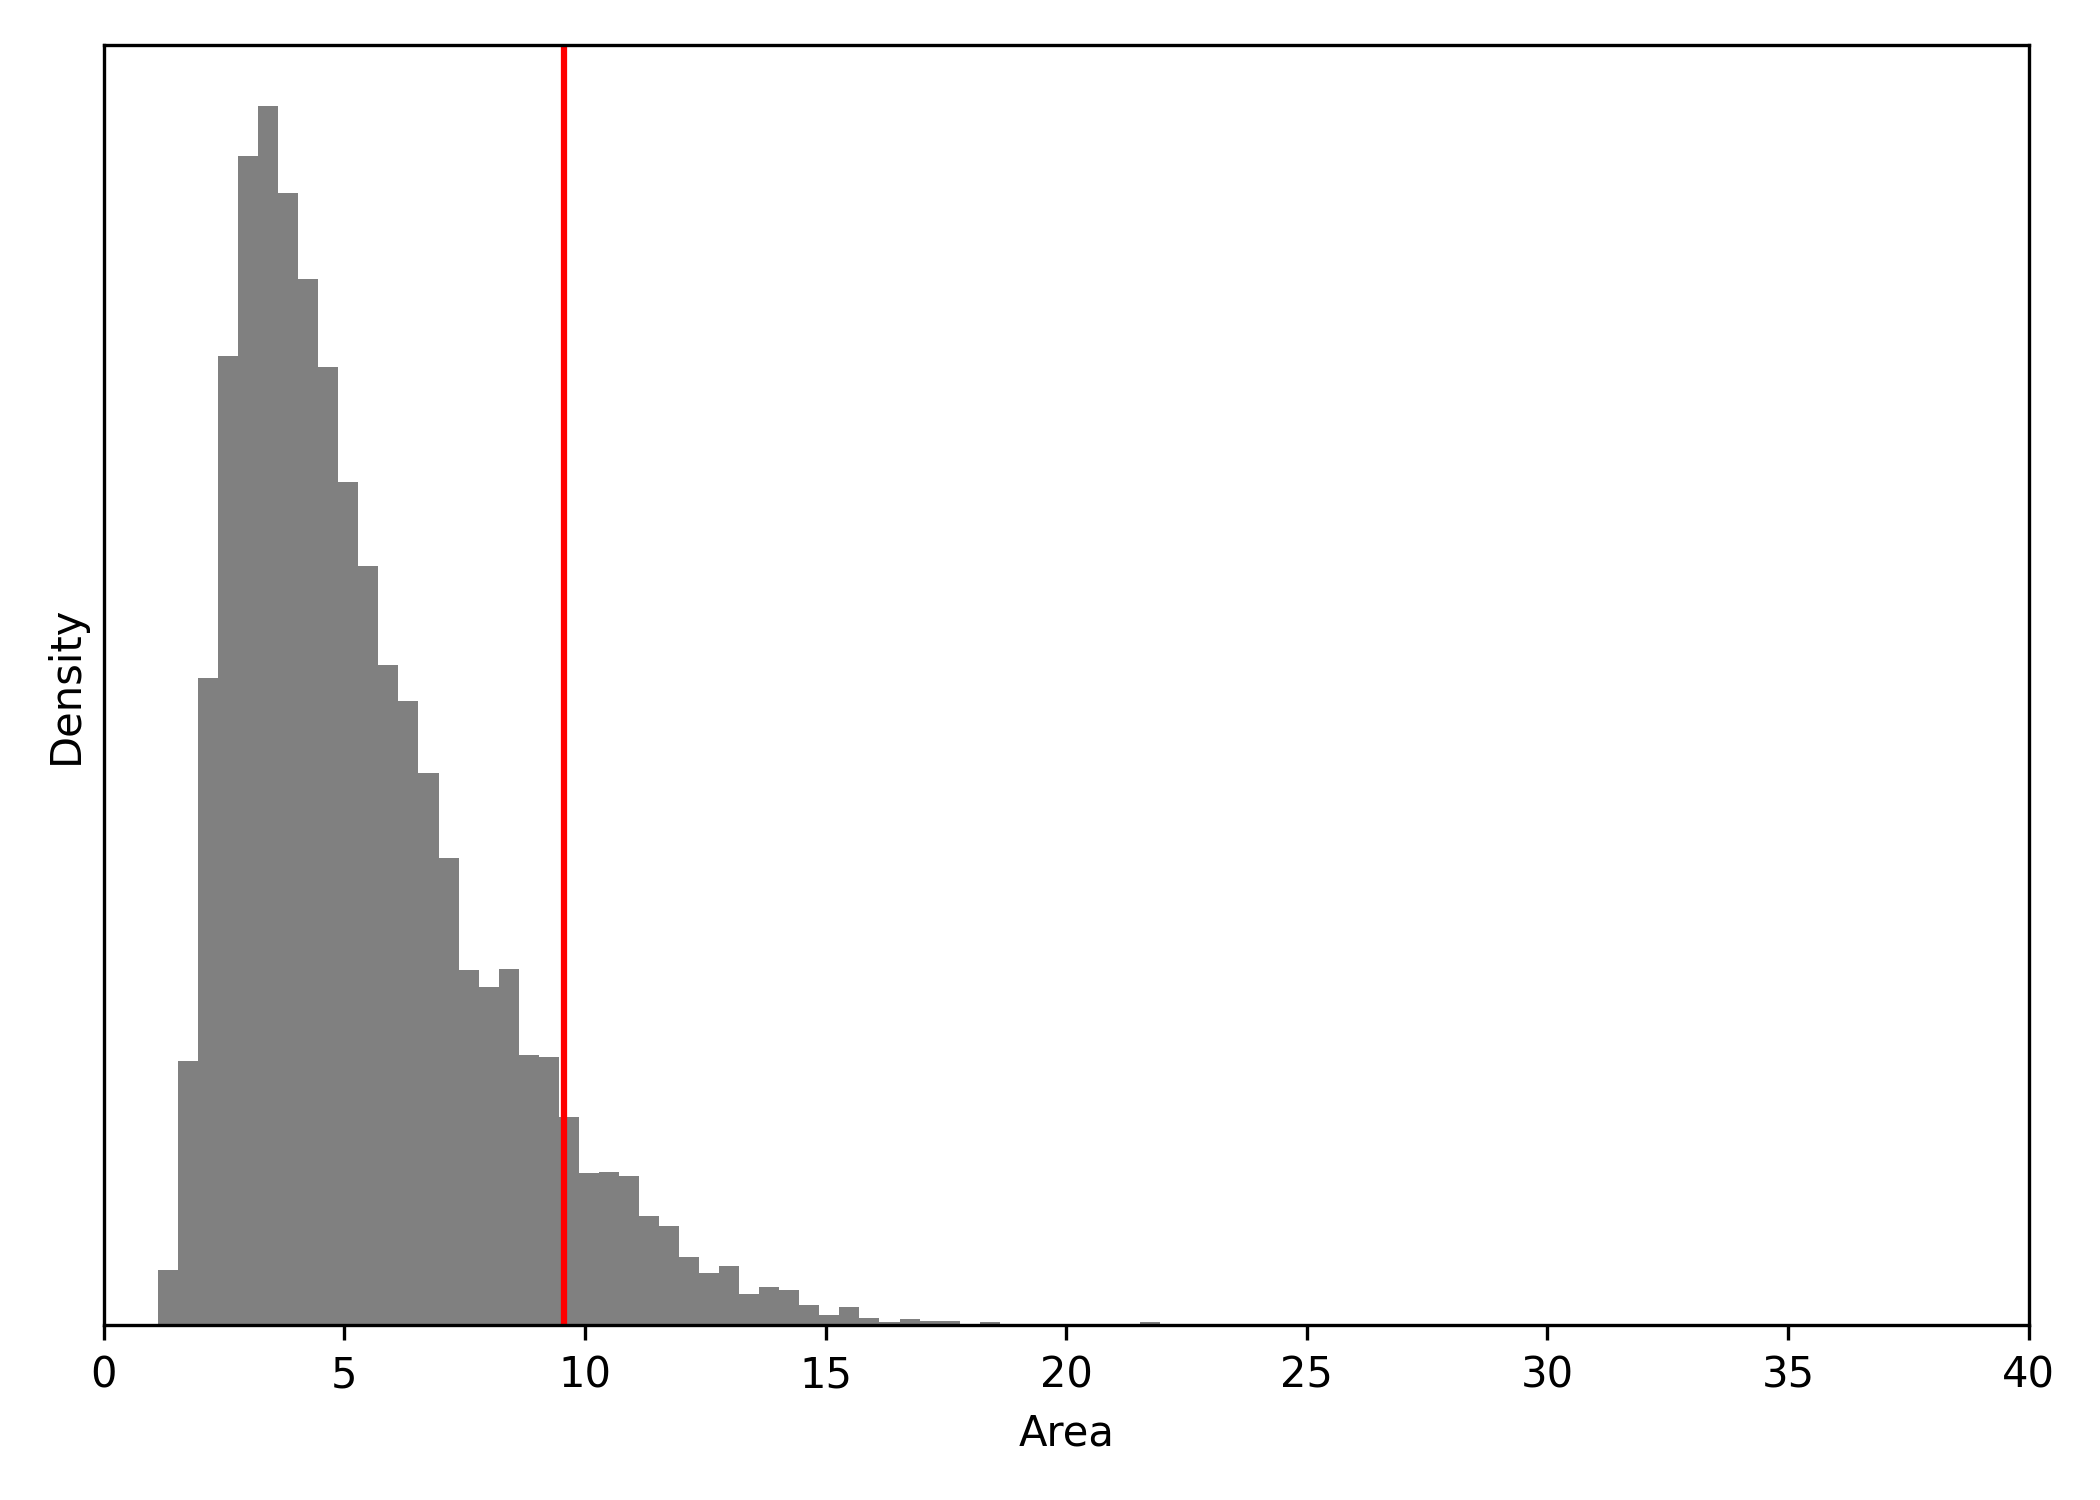
\includegraphics[scale=0.4]{images/diagnostic_test_rtrn.png}	
\end{frame}

\begin{frame}{Estimation: \blue{Triple} vs \red{Mono}}
	Estimator for parameter of interest\footnote[frame]{Variance estimator proposed in Breskin et al. (2021) \textit{SIM}}
	\[\hat{\psi}(t) = \left(\hat{F}_{320}^{\blue{3}}(t) - \hat{F}_{320}^{\violet{2}}(t)\right) + \left(\hat{F}_{175}^{\violet{2}}(t) - \hat{F}_{175}^{\red{1}}(t)\right)\]
\end{frame}

\begin{frame}{Comparison of interest}
	\centering
	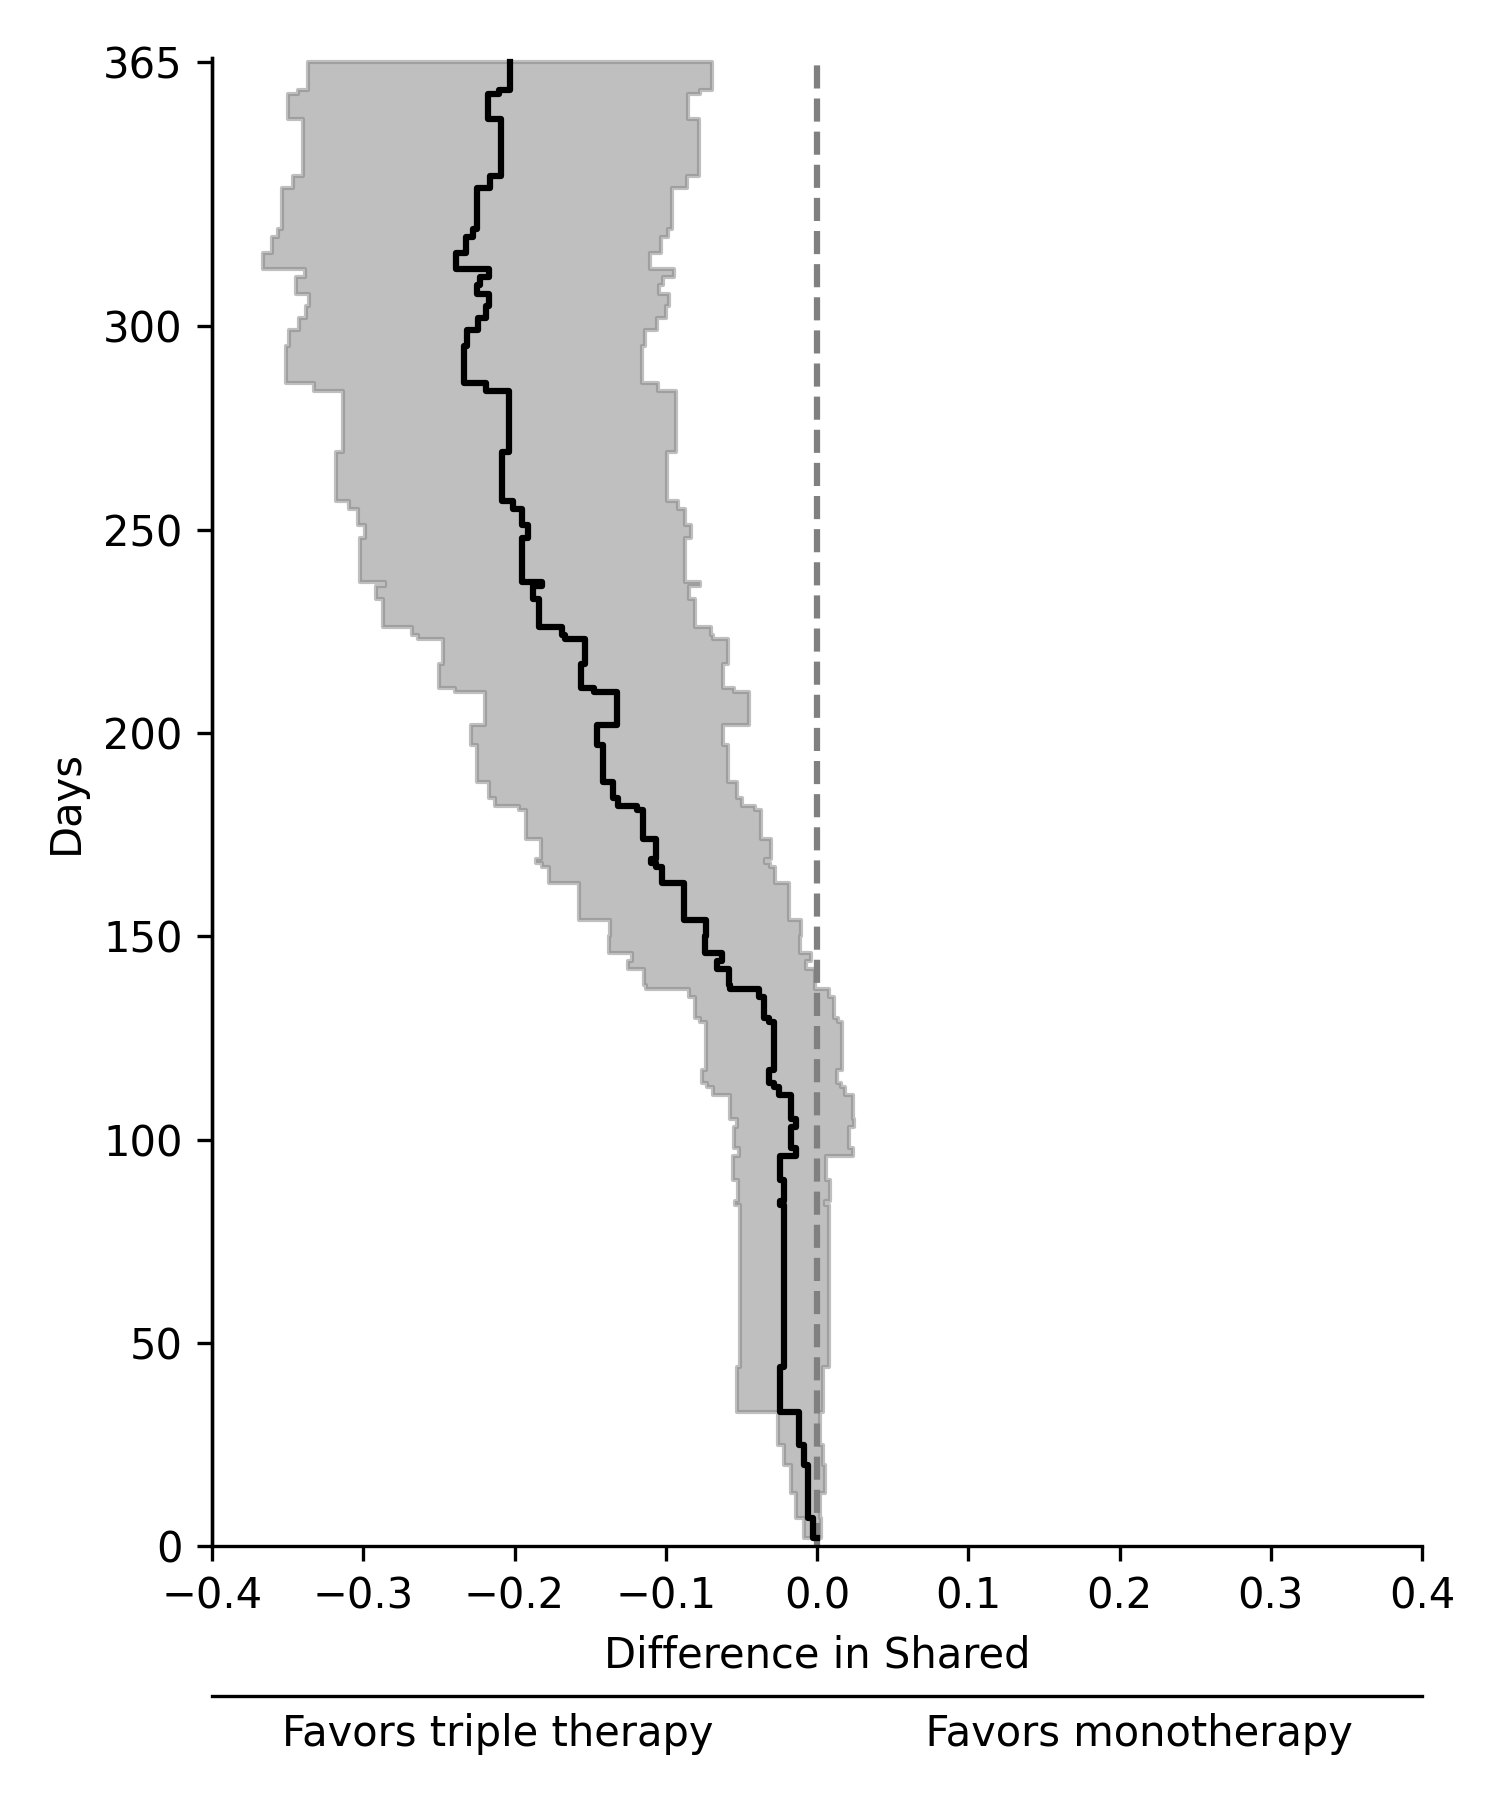
\includegraphics[scale=0.45]{images/results_twister.png}	
\end{frame}

\begin{frame}{Summary}
	Bridged comparisons offer
	\begin{itemize}
		\item Comparisons across trials
		\begin{itemize}
			\item Analytical corrections for differences
		\end{itemize}
		\item A testable condition
	\end{itemize}
\end{frame}

\section{Future Work and Extensions}

\begin{frame}{Ongoing Applications}
	Pre-exposure prophylaxis for the prevention of HIV
	\begin{itemize}
		\item \blue{TAF/FTC} vs \red{Placebo}
		\begin{itemize}
			\item Alternative tenofovir pro-drug
			\item Comparison 
			\begin{itemize}
				\item DISCOVER (\blue{TAF/FTC} vs. \violet{TDF/FTC})
				\item iPrEx (\violet{TDF/FTC} vs. \red{Placebo})
			\end{itemize}
		\end{itemize}~\\
		\item \blue{LA-CAB} vs \red{Placebo}
		\begin{itemize}
			\item Long-acting injectible
			\item Comparison 
			\begin{itemize}
				\item HPTN-083 (\blue{LA-CAB} vs. \violet{TDF/FTC})
				\item iPrEx (\violet{TDF/FTC} vs. \red{Placebo})
			\end{itemize}
		\end{itemize}
	\end{itemize}
\end{frame}

\begin{frame}{Statistical Models}
	\centering
	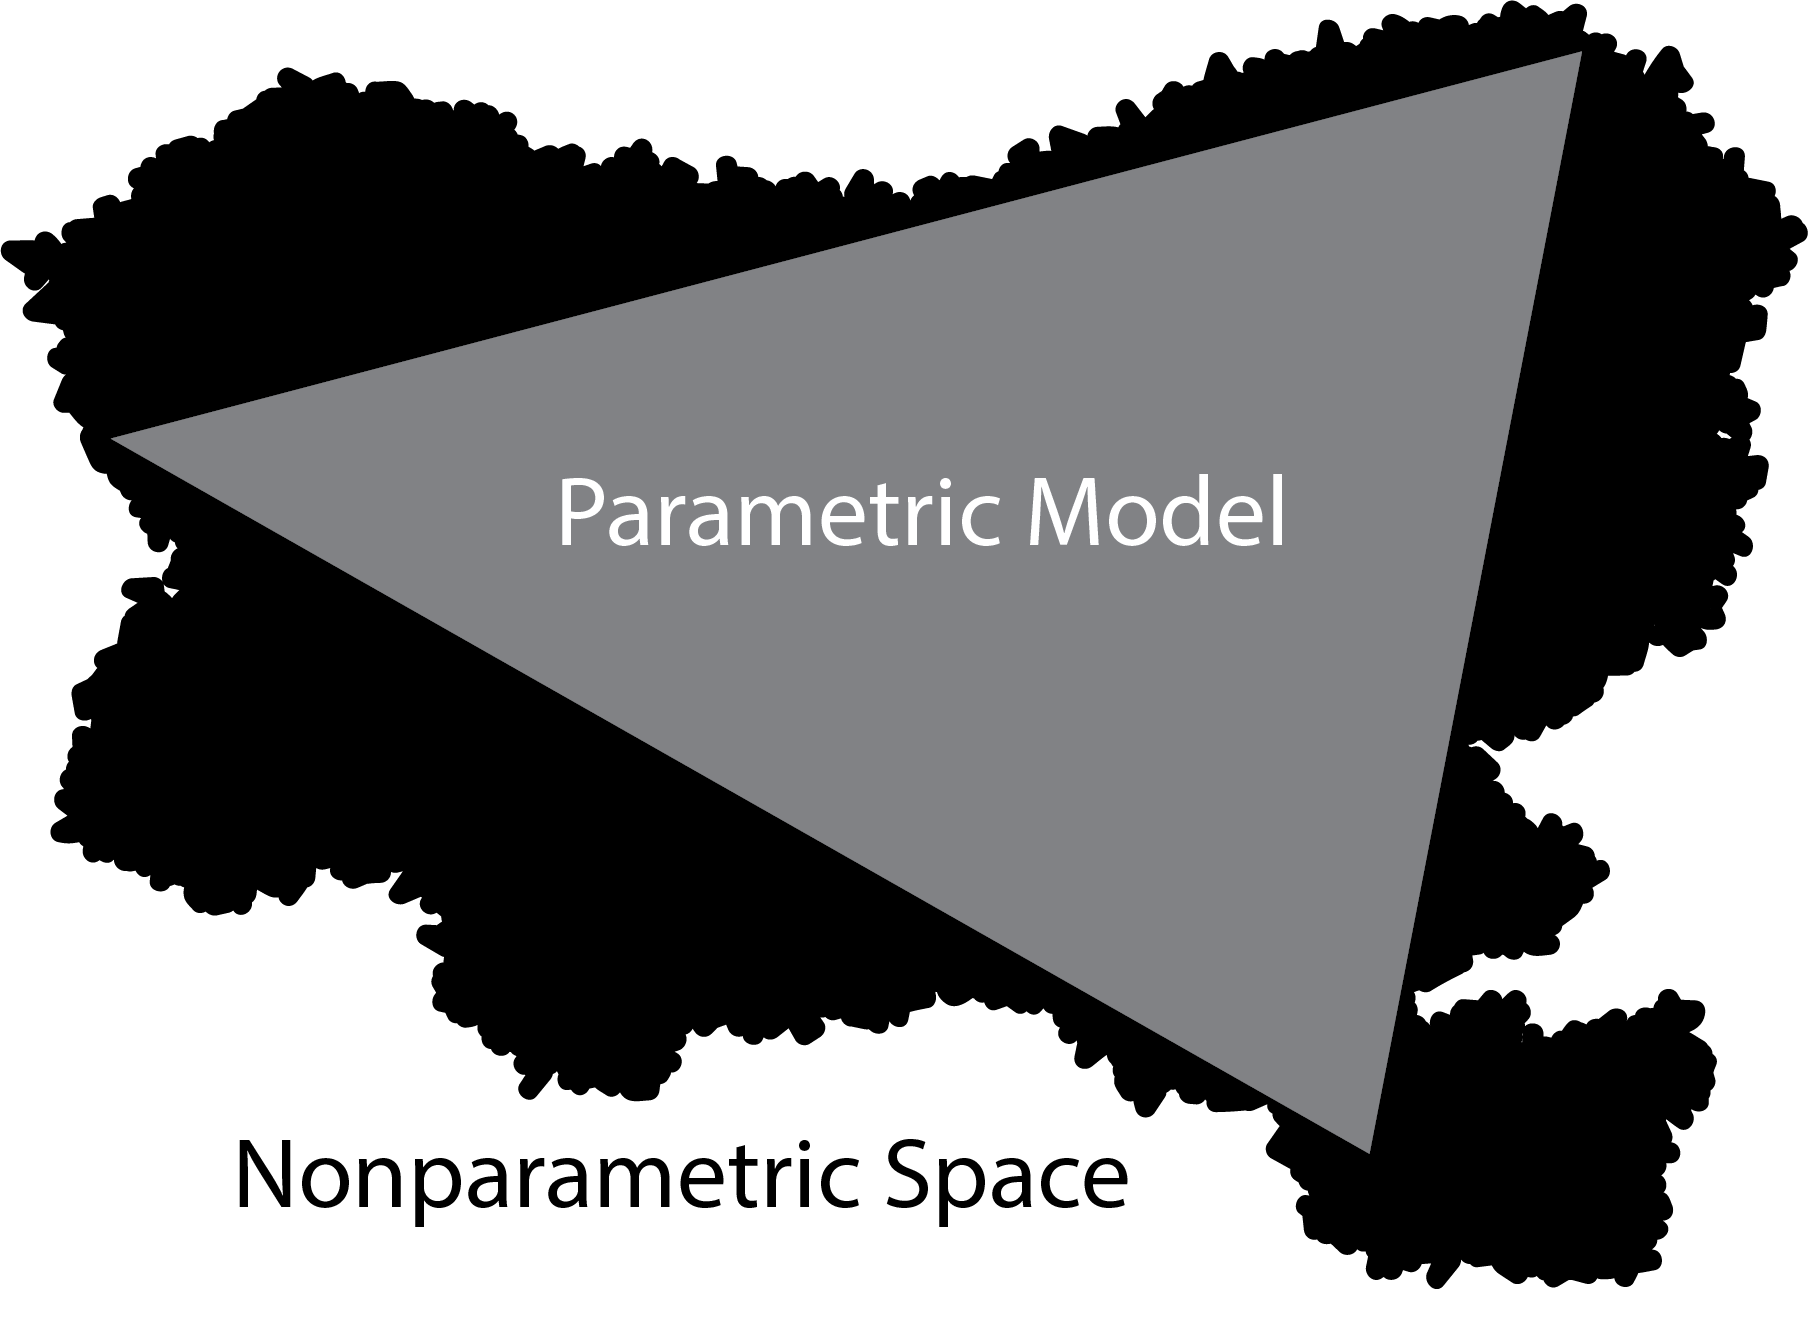
\includegraphics[scale=0.55]{images/parametric_model.png}
\end{frame}

\begin{frame}{Other Extensions}
	Nested studies\\~\\
	Measurement error
	\begin{itemize}
		\item Other corrective approaches
	\end{itemize}~\\
	Diverse data sources
	\begin{itemize}
		\item Subject-matter knowledge
		\begin{itemize}
			\item Semi-Bayes
		\end{itemize}
		\item Pharmacokinetic data
	\end{itemize}
\end{frame}

\section{Questions}

\section{Supplement}

\begin{frame}{Didactic Simulation: Setup}
	\begin{center}
		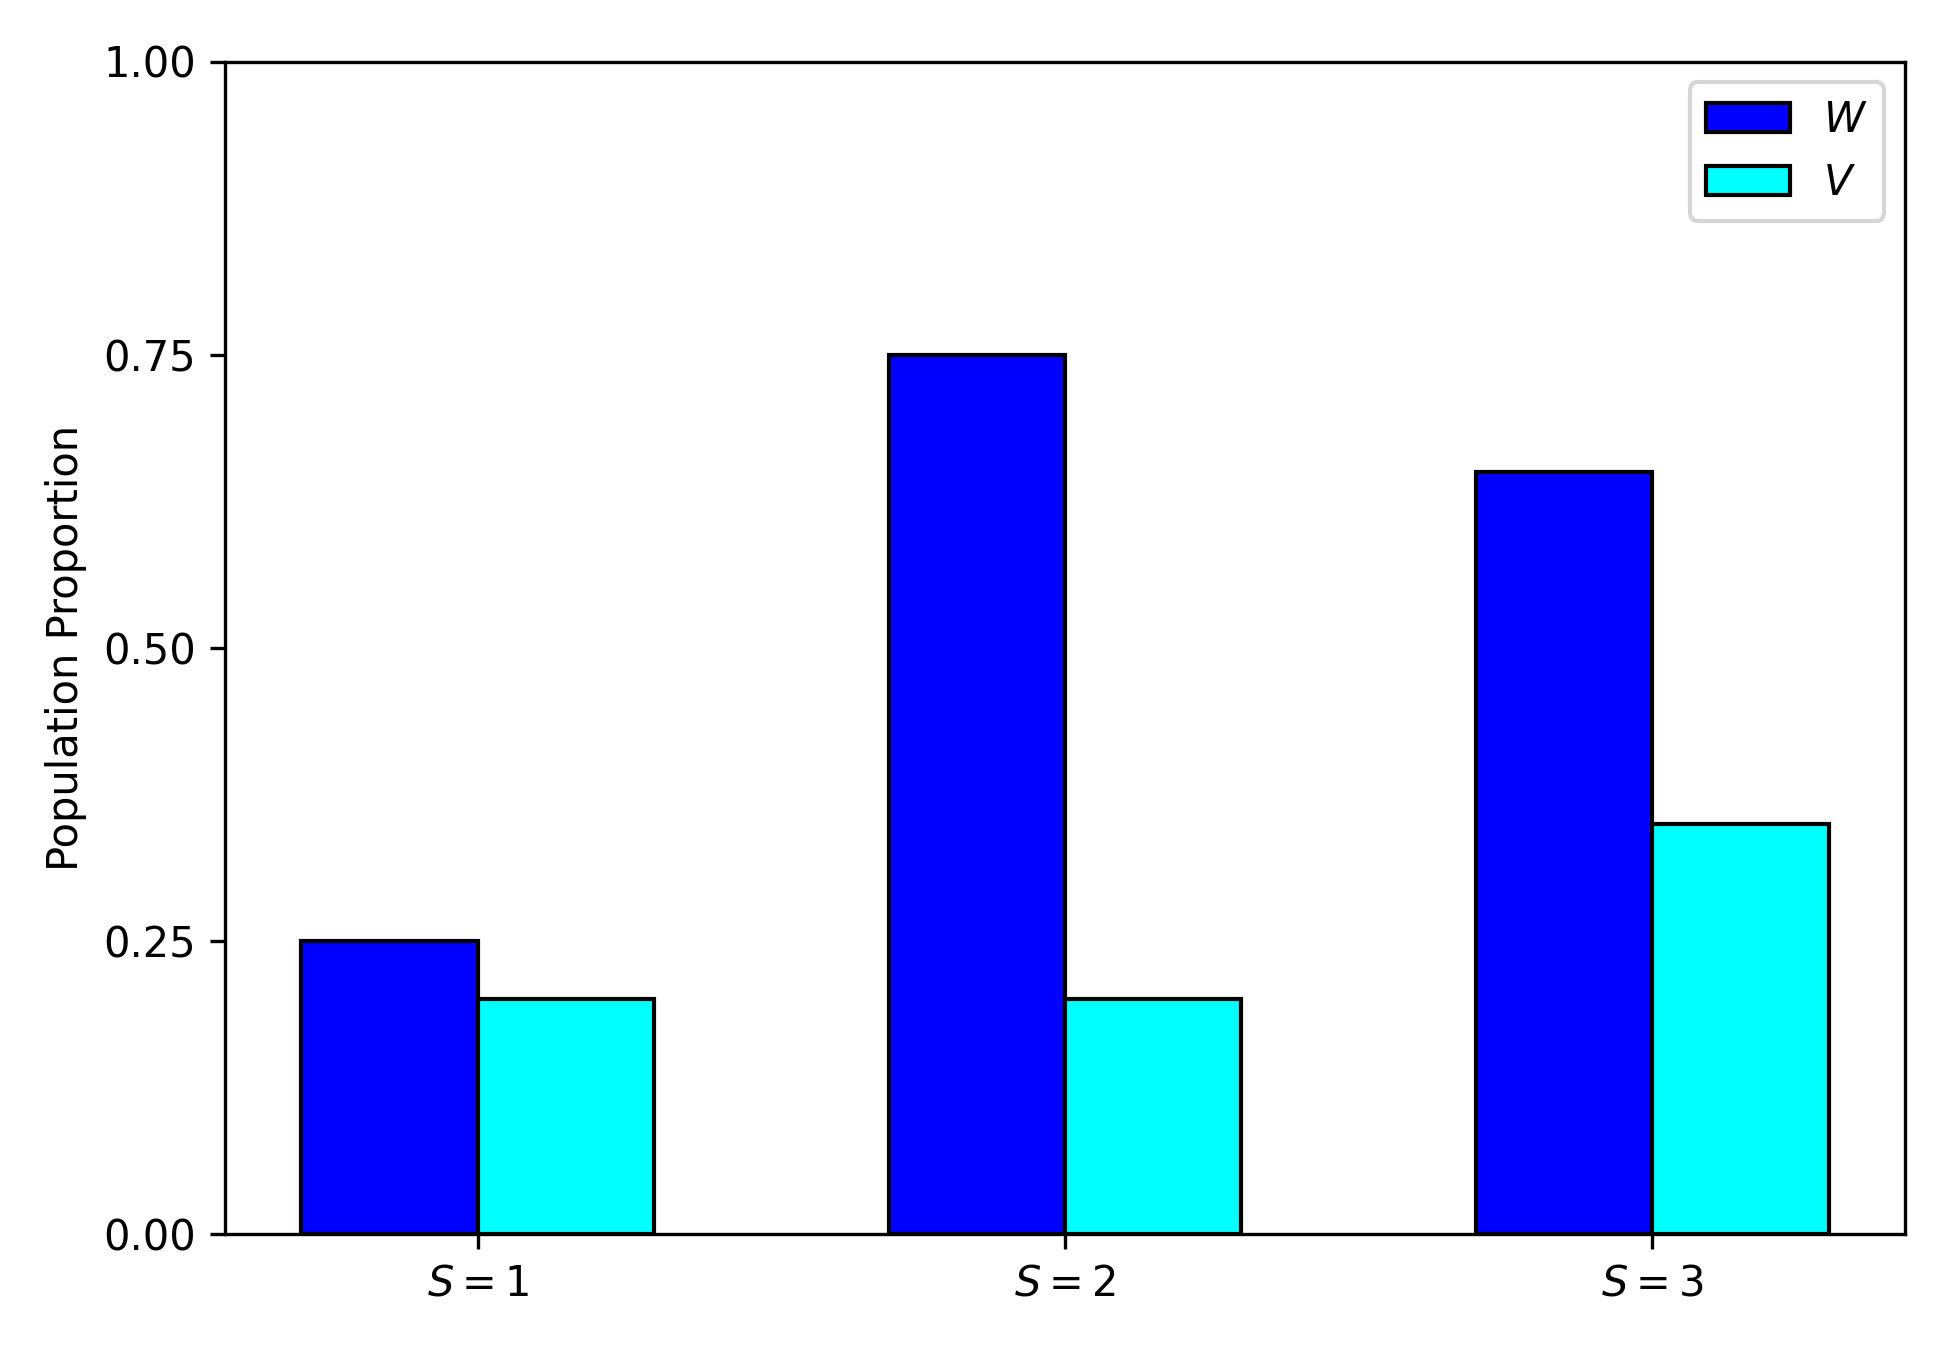
\includegraphics[scale=0.4]{code/figure_didactic_popprops.png}	
	\end{center}
	\[\Pr(Y | W,V) = \text{logit}(-0.5 + 2W - V - 2WV + \epsilon)\]
	\[\Pr(Y^* | Y) = 0.80 X + (1-0.95)(1-X)\]
\end{frame}

\begin{frame}{Didactic Simulation: Results}
	\centering		
	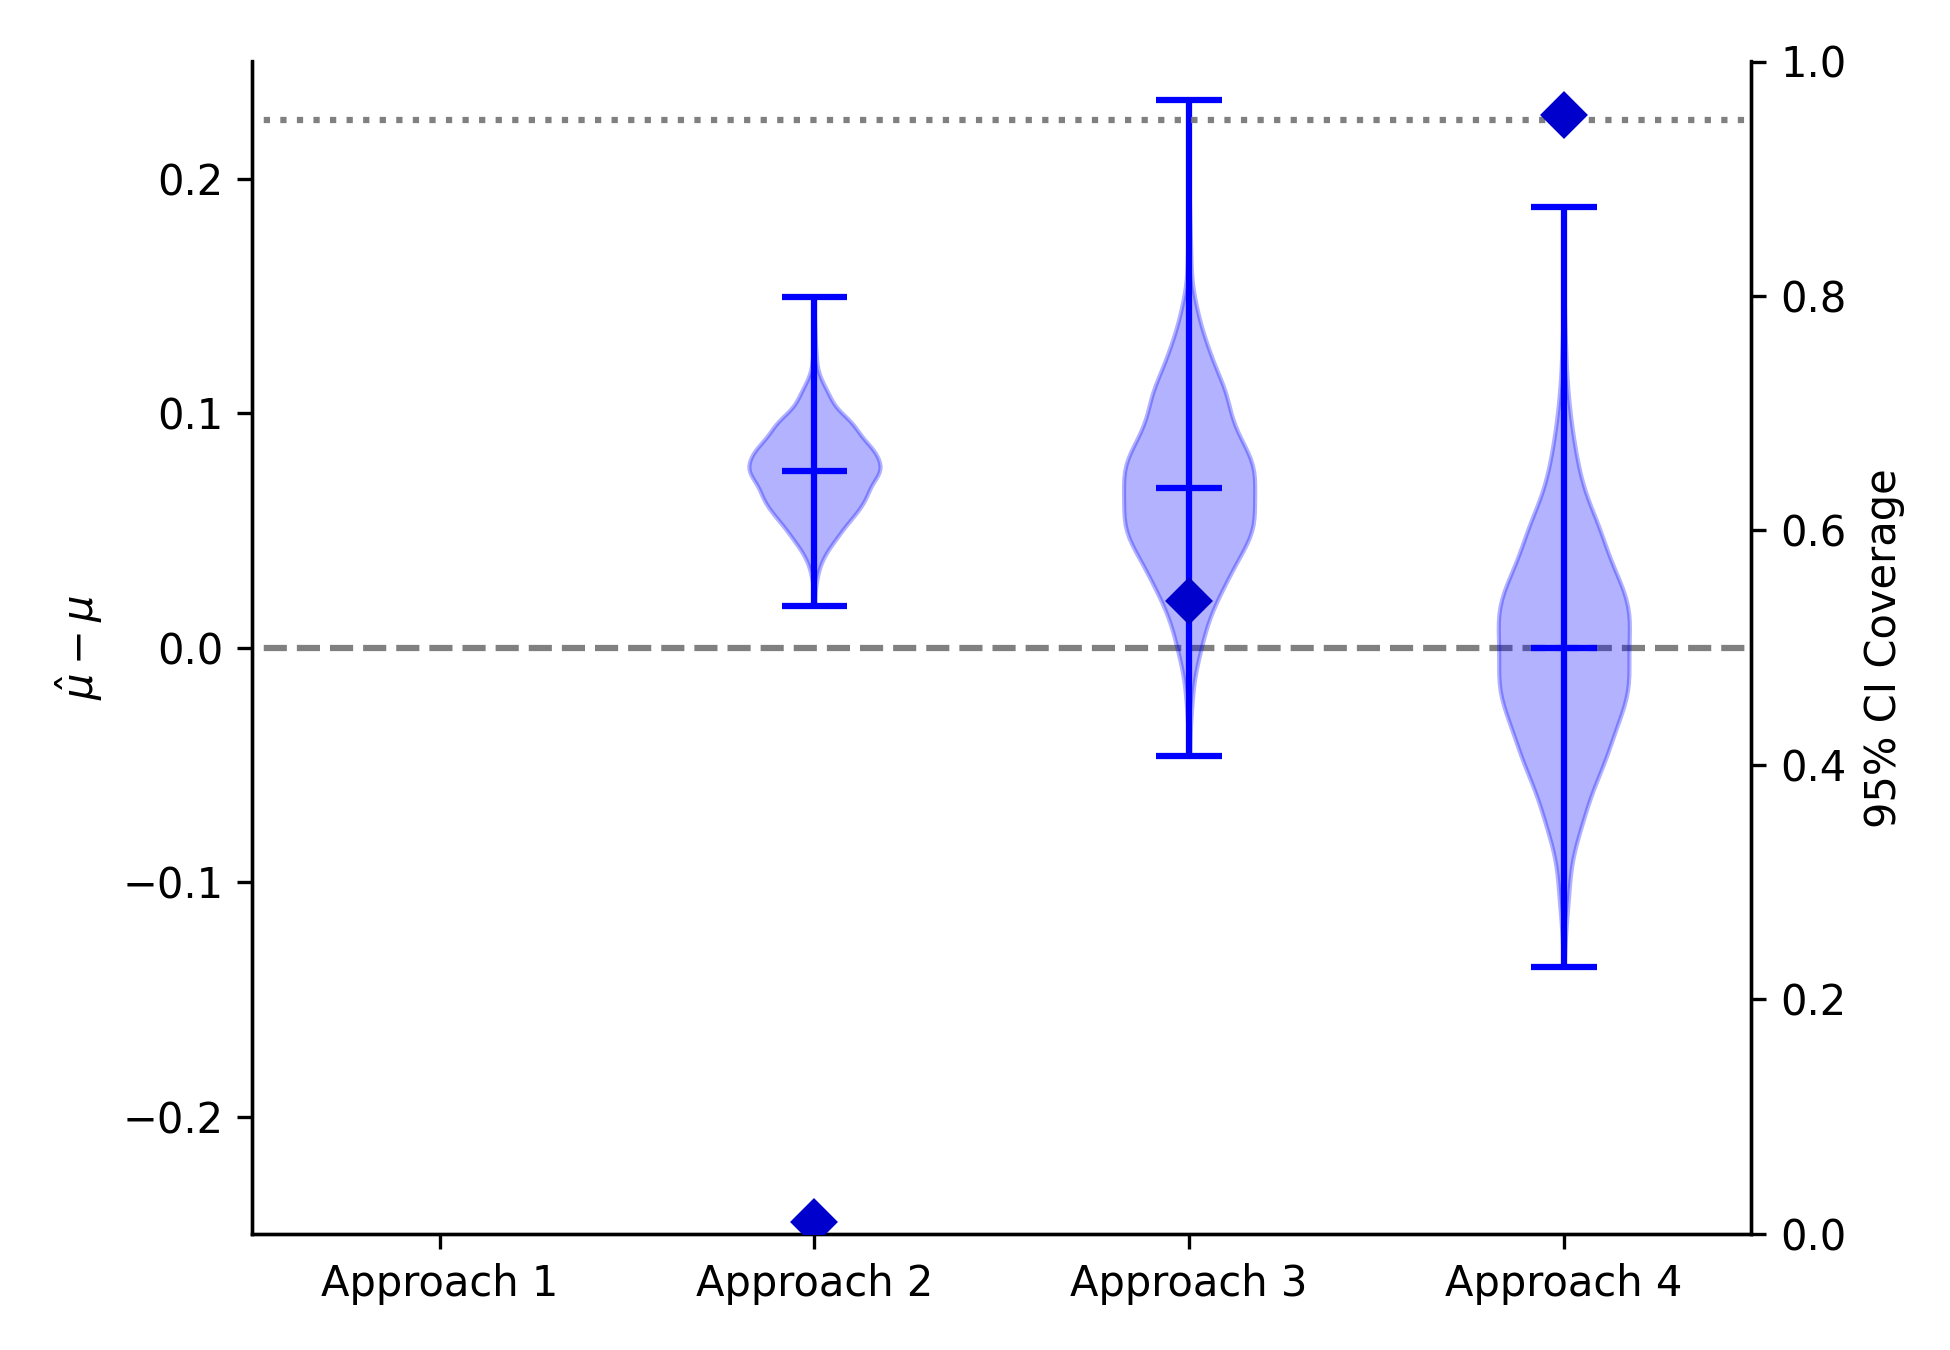
\includegraphics[scale=0.55]{code/figure_didactic_results.png}	
\end{frame}

\end{document}
